\documentclass[14pt]{extarticle}

\usepackage{amsmath, amsthm, amssymb}
\usepackage[boxed, lined]{algorithm2e}
\usepackage{CJKutf8}
\usepackage{float}
\usepackage{graphicx} 
\usepackage{hyperref}
\usepackage{makecell}
\usepackage{pythonhighlight}
\usepackage{subfigure}
\usepackage{tabularx}
\usepackage{url}
\usepackage[utf8]{inputenc}

\newtheorem{question}{Question}
\newtheorem{activity}{Activity}
\newtheorem{theorem}{Theorem}
\newtheorem{objective}{Objective}
\newtheorem{lemma}{Lemma}
\newtheorem{fact}{Fact}
\newtheorem{claim}{Claim}
\newtheorem{corollary}{Corollary}
\newtheorem{prop}{Proposition}
\newtheorem{conjecture}{Conjecture}
\newtheorem{definition}{Definition}
\newtheorem{obs}{Observation}

\textheight=22.5cm
\topmargin=-1cm
\oddsidemargin=5mm 
\textwidth=16cm

\pagenumbering{gobble}
\title{
\includegraphics{XJTLULOGO.png} \\ \vspace{20mm} Stable Marriage Problem and Algorithms\\ \vspace{10mm}
\begin{CJK*}{UTF8}{gbsn}
双边匹配及其算法
\end{CJK*}
\vspace{20mm}}
\date{\today}
\author{Yunhan Liu 1929224,
\\ Supervisor: Dr. Aistis Atminas, \vspace{20mm}
\\Financial Mathematics
\\Department of Mathematical Science \vspace{20mm} }

\begin{document}

\maketitle

\newpage 
.
\newpage

\begin{abstract}
  The stable marriage problem, which known as pairing $n$ man with $n$ woman, can be applied in many fields including mathematics, computer science, economics and game theory.
  In this report, two algorithms will be introduced and discussed to make a comparison between two primary goals including stable pairing and global optimal. 
  Also, the possible method will be given to make an improvement based on the two algorithms.
  \\
  \begin{CJK*}{UTF8}{gbsn}
    稳定婚姻问题是将$n$对候选人进行匹配的问题。
    其可被应用在众多领域,包括但不限于数学,计算机科学,经济学以及博弈论。
    在本文中,这个问题将被详细解释,并引入两个算法用于解决此问题在不同条件下的最优解。
    另外,本文还将提供其他可能的方法来提升原有算法的运行效率或减少原有算法的副作用。
  \end{CJK*}
  \\
  \\
  \\
  Key words: Gale-Shapley algorithm, Hungarian algorithm, Stable marriage problem.
  \\
  \\
  \\
  \\
\end{abstract}  

\newpage

\tableofcontents

\newpage

\pagenumbering{arabic}

\section{Introduction}

\subsection{Background}
Stable marriage problem concerns a system of forming stable pairs between elements from different sets, 
naturally arises in real-life practical problems including marriage, university admission, supply rationing and job assignment. 

In most of western country, the university admission system is set as follow: 
students send their materials to apply the universities. And each university may decide whom to accept according to the received materials and make offer to the candidates. 
However, there will be a problem: the applicants, who receive many offers, may choose some universities rather than others. 
So, for the viewpoint of universities, they have to make more offers than the places. 
But in this scenario, if universities make more offer than the place they have, then they have the risk of overcrowd of the programme.

Here, the model can be simplified as follow: the university have m positions of programmes and each candidate can finally get only one position. 
Also, there are n students who are expecting to apply for a position. 
Here it can be assumed that every student or university has a preference list. 
The goal is to find the matching, or in terms of graph theory is to find stable matching. 
Here the term “Matching” is temporarily defined as one-to-one pair of programme position and candidates. 
And the term “stable” is informally defined as there is no pair that the university and student both have a tendency of get a better choice according to the preference. 
(The terms mentioned above will be formally defined in section 1.4.) 

As examples like the case mentioned above is indeed important and widely existed in real life, the stable marriage has aroused interest in many fields of science, 
so that in 2012 Lloyd S. Shapley and Alvin E. Roth won the Noble Economic Prize for their great contribution from abstract theory on stable marriage problem to practical design of market institutions.

As one of classic cases, stable marriage problem can be used as a model, which is particularly suitable for describing two-sided matching. 
Although no one case can perfectly fit this model, with a few modifications, it can be widely applied to many bipartite matching problems and get satisfactory results. 

\subsection{Existing literature on stable marriage problem}
Stable marriage problem has applications in many fields, including mathematics, computer science, economics and game theory. 
It has been extensively studied in the literature and there have been many academic achievements given by different scholars and institutions, 
including mathematical theorems, algorithms, and applications over the past 7 decade.

In 1962, David Gale from Brown University and Lloyd Shapley from University of California, Los Angeles published the seminal paper entitled with “College Admissions and the Stability of Marriage” \cite{GS1962}. 
In the paper, Gale and Shapley gave an elegant algorithm named as “Gale-Shapley algorithm”, or “deferred acceptance algorithm”, to achieve stable matching and solve the problem of university enrollment and couple pair. 
Also, they proved the existence of the stable marriage in the paper. 
This is probably the earliest paper on stable marriage problem and stable matching. 

The Gale-Shapley algorithm is not the only algorithm of solving the problem. 
Earlier in 1955, by reduction from simple assignment problem to general assignmnet problem, an algorithm called Hungarian algorithm used to solve “assignment problem” (it can be treated as a variant of stable marriage problem) was raised by the Harold W. Kuhn \cite{Kuhn1955}. 
Compared to the Gale-Sharpley algorithm, it was revealed that Hungarian typically involves a larger number of pairs \cite{manlove2013}.
Also, in 1957, James Munkres reviewed the method and proved that the Hungarian algorithm is strictly polynomial \cite{Munkres1957}, so the algorithm is also called Kuhn-Munkres algorithm.
The original algorithm have a time complexity of $O(n^2)$. 
But later, in 1972, Edmonds and Karp improved the algorithm to a time complexity of $O(n^3)$ with some modifications \cite{Edmonds_Karp1972}.

The similar mechanism had been used 10 years before Gale and Sharpley’s paper launched \cite{GS1962}.
In a paper from 1984, Alvin E. Roth studied the algorithm used in the National Intern Matching Program in the United States, which is now named as National Resident Matching Program (NRMP). 
It provided a very similar algorithm related to the Gale-Sharpley algorithm. 
He assumed that the reason for the success of NRMP is to provide a stable matching \cite{Roth1984NRMP}. 
One year later, he examined the different between “college admission” problem and stable marriage problem \cite{Roth1985NotEqual} and proposed the conception of “2-sided matching” \cite{Roth1985bipartite} in other papers. 

In 1971, McVitie and Wilson \cite{McVitie&Wilson} reviewed the Gale-Shapley algorithm and introduced a new algorithm based on recursive. 
Based on the new recursive algorithm, by involving the {\it breakmarriage} operation, all stable solutions from man-oriented to woman-oriented can be generated once.

In 1989, a book entitled with “The Stable Marriage Problem: Structure and Algorithms” by the Dan Gusfield and Robert W. Irving was published \cite{Gusfield1989}. 
The book reviewed the basic underlying structure of stable marriage and its variants including hospital-resident and stable roommate problem and show why the structure is important in derivation of efficient algorithms for problems such as generating all stable matchings and finding stable matchings with additional useful properties.
And in 2013, David F. Manlove published a book named as “Algorithmics of Matching Under Preference” \cite{manlove2013}. The book can be seen as a newest update for many structural and algorithmic results for these matching problems mentioned in Gusfield and Irving’s work \cite{Gusfield1989}.

\subsection{Methodology}
The aim of the study is to review the underlying structure of stable marriage problem, 
compare between different algorithms, and explorer the different variants and their applications. 

The method utilized for this report are a combination of literature research, qualitative research and quantitative research. 
Refer to the exist literature, the stable marriage problem was constructed by the mathematical expression. 
After that, proofs were given to prove the existence of stable solutions. 
And the different algorithms aiming at getting the stable pairs were given. 
For algorithm analysis, the coding was done by using python as there are many packages and supportive resources.
Both time complexity and accuracy were considered. 
There were questions random generated and solved by the different algorithms. 
The duration and accuracy were compared to quantitatively analyze the performance of the algorithm.

\subsection{Outline of the report}
The organization of the report is structured as follows: 
\begin{itemize}
  \item In section \ref{SMPintro}, the brief introduction to matching, stable marriage problem and its two primary goals will be given.
  \item In section \ref{variants and algorithms}, the underlying logic of two algorithms will be introduced to solve stable marriage problem and cover its two primary goals.
  \item In section \ref{performance_analysis}, the algorithms will be tested with python program. the improvement of the algorithms will also be included.
\end{itemize}

\section{Stable marriage problem} \label{SMPintro}

In this section, the primary conceptions will be introduced to construct the foundation for more detailed research. 
The general notation and terminology will be given to show the underlying results of the stable marriage problem. 
Also, the report will explore more detailed information of each topic.

\subsection{Matching in graph}

In this subsection, the fundamental definitions, together with theorems and structural results of the graph will be given to 

Let graph $G=(V,E)$ be a graph, consisted with the set of vertices $V$ and the set of edges $E$. 
\begin{definition}
  (bipartite graph) 
  The graph $G$ is bipartite if its vertices can be partitioned into two disjoint sets $L$ and $R$ such that:
  \begin{itemize}
    \item Every edge of $G(V,E)$ connects a vertex in $L$ to a vertex in $R$.
    \item i.e., no edge connects two vertices from the same part.
  \end{itemize}
  $L$ and $R$ are called the {\it parts} of $G$.
\end{definition}

\begin{figure}[H]
  \centering
  \subfigure[]{
    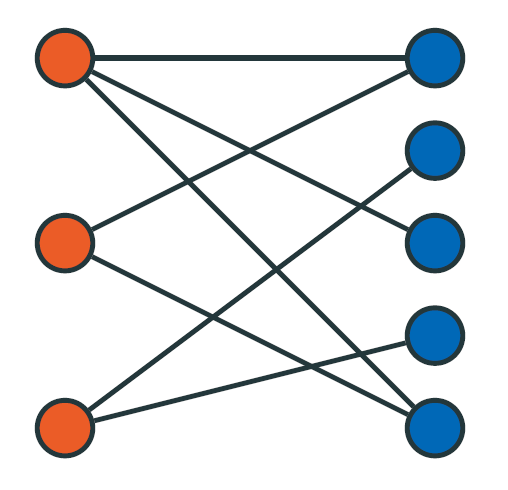
\includegraphics[width=0.37\textwidth]{Bipartite1.png}
  }   
  \quad
  \subfigure[]{
    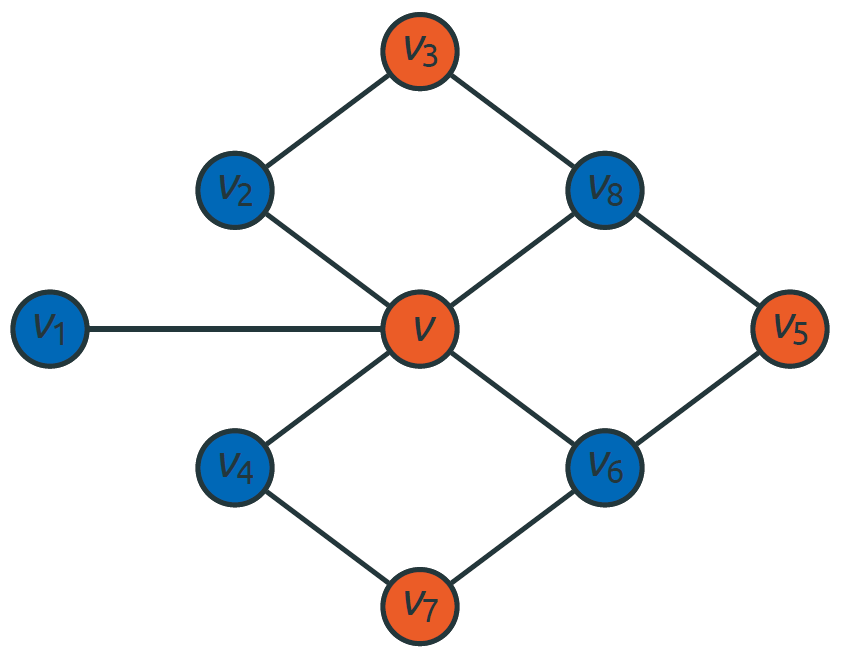
\includegraphics[width=0.37\textwidth]{Bipartite2.png}
  } 
  \caption{Two different forms of bipartite graph \cite{coursera}.}
\end{figure}

And {\it matching} in graph is defined as:

\begin{definition}
  (matching)
  A matching in a graph $G(V,E)$ is a set of edges without common vertices.
\end{definition}

\begin{definition}
  (maximum matching)
  A maximum matching is a matching of the largest size.
\end{definition}

\begin{definition}
  (perfect matching)
  A perfect matching is a set of edges that is a one-to-one correspondence between the parts of a bipartite graph with parts of equal size.
\end{definition}

\begin{figure}[H]
  \centering
  \subfigure[Bipartite graph]{
    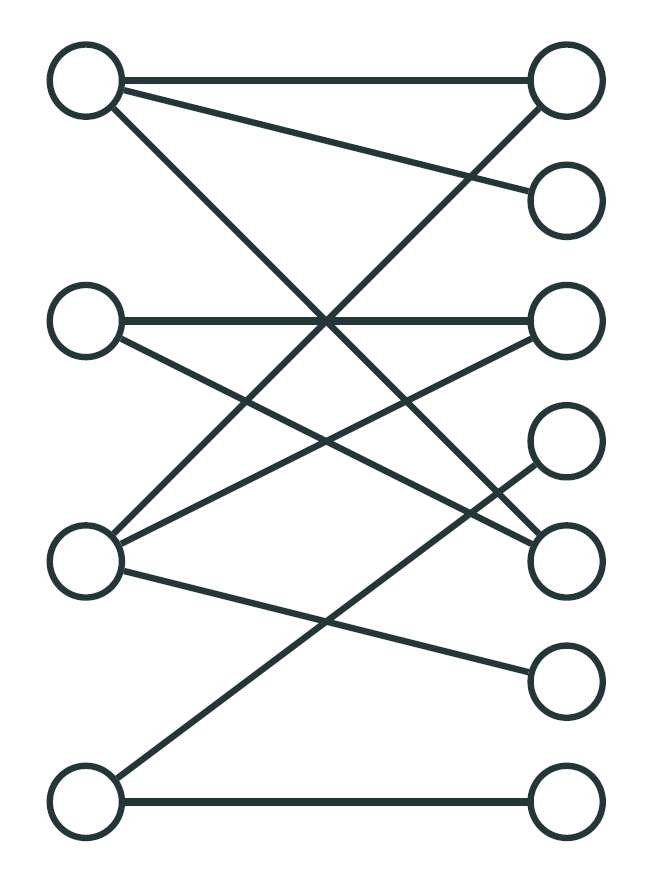
\includegraphics[width=0.25\textwidth]{matching1.png}
  }   
  \quad
  \subfigure[Matching]{
    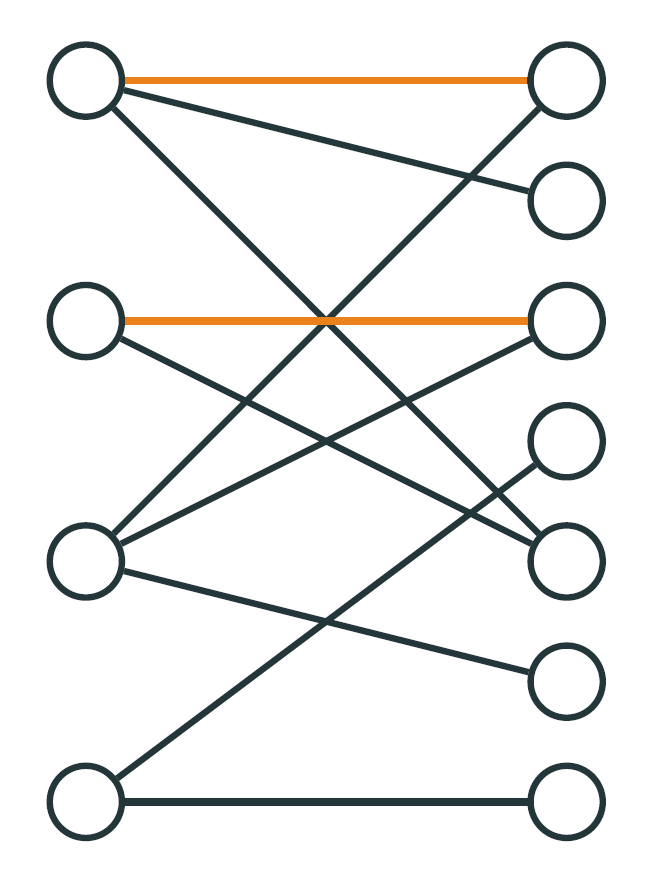
\includegraphics[width=0.25\textwidth]{matching2.png}
  } 
  \quad
  \subfigure[Maximum matching but not perfect matching]{
    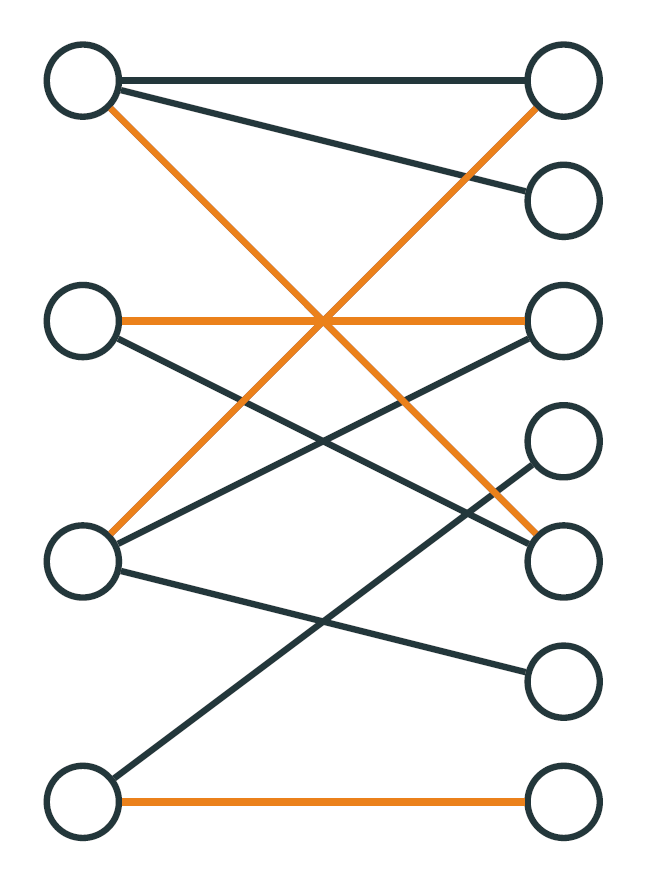
\includegraphics[width=0.25\textwidth]{matching3.png}
  } 
  \caption{Bipartite, matching and maximum matching \cite{coursera}.}
\end{figure}

It can be seen that the maximum matching is not usually perfect matching.
But the perfect matching is always maximum matching.
To find a matching in $G$ with as many edges as possible, the definition of {\it alternating path} and {\it augmenting path} come with follow:

\begin{definition}
  (alternating path)
  A path in $G(L\cup R,E)$ which starts in left part $L$ at an unmatched vertex and then contains, 
  alternately, edges from $E\backslash M$ and from $M$, is an alternating path with respect to $M$ (given in \ref{alternating_and_augmenting_path}).
\end{definition}

Note that the path is allowed to consist of its starting vertex only. And:

\begin{definition}
  (augmenting path)
  An alternating path $P$ that ends in an unmatched vertex of $R$ is called an augmenting path (given in \ref{alternating_and_augmenting_path}).
\end{definition}

\begin{figure}[H] \label{alternating_and_augmenting_path}
  \centering
  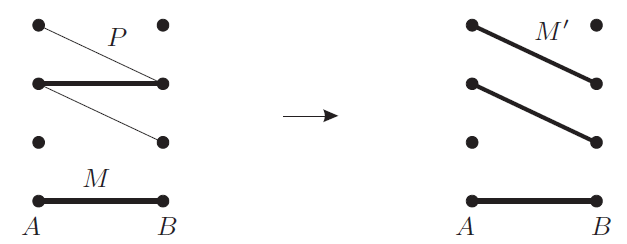
\includegraphics[width=0.7\textwidth]{alternating_and_augmenting_path.png}
  \caption{Augmenting the matching M by the alternating path P\cite{Diestel2017}.}
\end{figure} 

Here, by finding augmenting path until no more improvement can be found, there will always be an optimal matching obtained.
Therefore, the problem of finding optimal matchings transfers to the problem of finding augmenting paths.

Before getting into the first theorem, the definition of (vertex) cover is given by:

\begin{definition}
  (vertex cover)
  A vertex cover of a graph $G$ is a set of vertices $C$ such that every edge of $G$ is connected to some vertex in $C$.
\end{definition}

Then the \textbf{K$\ddot{o}$nig's theorem} comes as follow:

\begin{theorem}
  (K$\ddot{o}$nig's 1931)
  In a bipartite graph $G$, the maximum cardinality of a matching is equal to the minimum cardinality of a vertex cover of its edges.
  i.e. the number of edges in a maximum matching equals the number of vertices in a minimum vertex cover.
\end{theorem}  

\paragraph{Proof.} 
Let $M$ be a matching in $G$ of maximum cardinality. 
From every $M$ edge in $M$, choose one of its ends: its end in $B$ if some alternating path ends in that vertex, and its end in A otherwise (given in \ref{konig_proof}). 
It would be proved that the set $U$ of these $\lvert M \rvert$ vertices covers $E$; 
since any vertex $U$ cover of $E$ must cover $M$, there can be none with fewer than $\lvert M \rvert$ vertices,
and so the theorem will follow.
(end of proof)

\begin{figure}[H] \label{konig_proof}
  \centering
  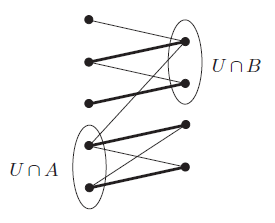
\includegraphics[width=0.35\textwidth]{konig's_proof.png}
  \caption{The vertex cover $U$ \cite{Diestel2017}}
\end{figure}

These definitions, together with K$\ddot{o}$nig's theorem, constructs the theoretical basis for the Hungarian algorithm, which will be mentioned in section \ref{hungarian}.

In our present case of a bipartite graph, more general case will be investigated when $G$ contains a matching of $L$.
When $\lvert L \rvert = \lvert R \rvert$, there will be easiler to achieve the perfect matching.
Hall's theorem (1935) provides a necessary and sufficient condition for graph $G(V,E)$ to admit a perfect matching.
Before that, some additional terminology will be given:

\begin{definition}
  (neighborhood) 
  Let $G(V,E)$ be a graph, and $S\subseteq V$ be a subset of vertices. 
  The neighborhood $N(S)$ of $S$ is the set of all vertices connected to at least one vertex in $S$.
\end{definition}

Then the \textbf{Hall's theorem} comes as follow:

\begin{theorem}
  (Hall 1935)
  In a bipartite graph $G=(L \cup R, E)$, the graph contains a matching of $L$ if and only if $\lvert S\rvert \leq \lvert N(S)\rvert$ for all $S \subseteq L$.
\end{theorem}

\paragraph{Proof.} It can be proved by induction on $\lvert L \rvert$. 
If $\lvert L \rvert = 1$, $1 = \lvert L\rvert \leq \lvert N(L)\rvert$, so there is a matching of size 1.
The induction hypothesis is: the statement holds for all graphs with smaller $\lvert L \rvert \leq k$.
It is needed to prove the statement for $\lvert L \rvert = K + 1$: pick a vertex $v \in L$ and its neighbor $u \in R$. 
If there is a matching on $L \backslash \{v\}$ and $R \backslash \{u\}$, proved.
Else if there is no matching on $L \backslash \{v\}$ and $R \backslash \{u\}$, 
then there is a set $S_1 \subseteq L \backslash \{v\}$ s.t. its neighbourhood in $R \backslash \{u\}$ is $<\lvert S_1 \rvert$. 
Then its neighborhood $T_1$ in $R$ is of size exactly $\lvert S_1 \rvert$.
There is a matching between $S_1$ and $T_1$, remove it.
In the remaining graph, every set $S\subseteq L$ has at least $\lvert S \rvert + \lvert S_1 \rvert - \lvert T_1 \rvert = \lvert S \rvert$ neighbors, there is a matching.
(end of proof)

\subsection{Stable marriage}
After foundation constructed, it is time to move on to the main topic.
Stable marriage problem is trying to such a situation: Consider there are two sets with the same number of $m$ men and $w$ women, each person has a preference list ordering all the candidate with the different gender.
It is wished to determine a matching of men $m_i$ and women $w_j$ with all person are married to one and only one person who has a different gender.

It seems that there must be an obvious solution by pair them according to their preference lists. 
But there may be some complicated issue beyond the first sense.
A simple example (given in \cite{physicist}) with the following preference list table.
\begin{table}[H] \label{stable_marriage_example}
  \center
  \begin{tabular}{|c|c|c|c|}
    \hline
    Man & Preference list & Woman & Preference list \\
    \hline
    \hline
    $m_1$ & $(w_1, w_2, w_3)$ & $w_1$ & $(m_3, m_1, m_2)$ \\
    \hline
    $m_2$ & $(w_1, w_3, w_2)$ & $w_2$ & $(m_1, m_2, m_3)$ \\
    \hline
    $m_3$ & $(w_2, w_3, w_1)$ & $w_3$ & $(m_3, m_2, m_1)$ \\
    \hline
  \end{tabular}
  \caption{Example: preference list table \cite{physicist}}
\end{table}
A scenario of {\it unstable} should be avoid and here comes with the definition of {\it unstable}:
\begin{definition}
  (unstable)
  A pair of couple will be called unstable if there are two candidates $m_1$ and $m_2$ are married with $w_1$ and $w_2$ but $w_1$ prefer $m_2$ and $w_2$ prefer $m_1$.
\end{definition}
\begin{figure}[H]
  \centering
  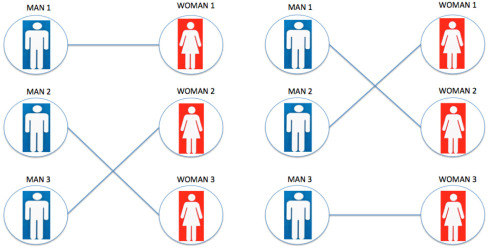
\includegraphics[width=0.8\textwidth]{stable_unstable.jpg}
  \caption{stable (left) and unstable (right) solution \cite{physicist}}
\end{figure}
Here, an obvious question is raised: will it always be possible to find a stable matching?
The formal proof for the question will be given later. 
And now, the optimal solution will be given according to Gale and Shapley's paper \cite{GS1962}.
\begin{definition}
  A stable matching is called optimal if every man is at least as well off under it as under any other stable matching.
\end{definition}  

\subsection{Global optimal solution}

As mentioned above, the purpose of stable marriage is to get the stable states for every candidate.
However, in many practical problems, the stable marriage model is not completely suitable. 
Another interesting state is maximize the total benefit, especially in game theory and economics. 
It concerns not only personal welfare (or {\it "Nash equilibrium"} in ecomonics), but also global optimal.
Specifically, individual stable makes sure that all candidates can get personal happiness, which can be also recognised as a kind of natural statement, or {\it "laissez-faire"} statement.
And global optimal may cannot satisfy everyone in the market. 
It gives suboptimal solutions for candidates but optimal solutions for the group or society.

Here, a question about this can be raised: is it possible to achieve both of the goals at the same time? 
Back to the example given in subsection \ref{stable_marriage_example}, 
it is not difficult to say that the global optimal solution $M = \{(m_1, w_2),(m_2,w_1),(m_3,w_3)\}$ provides a highest total satisfaction for all candidates. 
Here the total satisfaction is $S_{total} = \Sigma S_{m_i} + \Sigma S_{w_i} = 7 + 7 = 14$.
And for man-oriented solution $M = \{(m_1, w_1),(m_2,w_3),(m_3,w_2)\}$, the satisfaction is $S_{total} = 8 + 5 = 13$.
It can be also noticed that the global optimal solution contains pair: the pair $(m_1, w_1)$. 
For both $m_1$ and $w_1$, they have better choice than their current spouse.
However, the divorce of $m_1$ and $w_1$ could increases their individual satisfaction, but decreaseing overall satisfaction in the system.
Therefore, it might not be realistic to achieve both of the goals at the same time.

Another question is that: is there a quantitative standard to compare between two goals.
Fortunately, the answer is existed and is available.
Both of the problem can be solved by the algorithms with polynomial time. 
Individual stable and global optimal will also be two primary goals in the following investigations.

\section{Algorithms for stable marriage problem} \label{variants and algorithms}

In this section, two different algorithms will be introduced in order to solve the problem.
The background will be firstly introduced, followed with the pseudocodes to explain underlying logic of the algorithms.
Also, some related theorems and facts will be given and proved.

\subsection{Gale-Shapley algorithm}

The reason of necessity of involving the algorithms is that when $n$ is sufficiently large, it is not realistic to come through all possible solutions (i.e., brute-force) as the time complexity is $O(n!)$. 
One of the smart algorithms capable of finding a particular stable solution is the Gale-Shapley (GS) algorithm given by David Gale and Lloyd S. Shapley \cite{GS1962}.

\subsubsection{Underlying logic}

Warning: There is no claim about real life. The report respects the right of vulnerable groups and minorities. 
There are two kinds of algorithm: man-oriented and woman-oriented. The two versions will cause same outcome. 
For simplicity, the report will show only the man-oriented version. 

The algorithm follows these steps:

\begin{algorithm}[H]
  \SetAlgoLined
  Begin with every man and woman being free\;
  \While{there exists an unmarried man:}{
      The man $m_i$ proposes to the woman $w_j$, who ranks highest on his preference list and is not ever proposed\;
      \If{the women $w_j$ is not married with other}
        {then the man $m_i$ and women $w_j$ will engaged}
      \ElseIf{there is another man $m_k$ temporary engaged with woman $w_j$ and she prefers $m_k$ to $m_i$}
        {then the woman $w_j$ will rejects the $m_i$.}
      \Else{there is another man $m_k$ temporary engaged with woman $w_j$ and she prefers $m_i$ to $m_k$}
        {the $m_k$ will be abandoned and the man $m_i$ and women $w_j$ will engaged.}
    }
\end{algorithm}

The code is available in appendix \ref{GS_algorithm}.
The example mentioned above indicates the solution of the stable marriage can be always exist \cite{GS1962}.
\begin{theorem}
  (existance of stable matching)
  There always exiats a stable set of marriages
\end{theorem}  
\paragraph{Proof of Stability:} This can be proved by contradiction. If $(m,w)$ is an unstable pair, there must be a $w$ better than $w'$, the current partner of $m$.
So, $w$ have a higher rank than $w'$ in $m$'s preference list. That means $w$ rejected $m$ at previous round, i.e., $m'$ is better than $m$. 
That is contradict with the condition of {\it unstable}.    (end of proof)

It can also be proved that the algorithm provides optimal matchings to the "propose side". 
In stable marriage problem, it can be seen as "man-oriented" or "unfair to the women" while in college admission it can be seen as "candidate-oriented".
\begin{theorem}
  (optimality)
  Every applicant is at least as well off under the assignment given by the deferred acceptance procedure as he would be under any other stable assignment.\cite{GS1962}
\end{theorem}
\paragraph{Proof of Optimality:} Claim: if $m$ was rejected by $w$ during the algorithm, $(m,w)$ cannot appear in a stable matching.
This can be proved by induction by the rejection moment. It can be assumed that $(m,w)$ is a stable pair. But $w$ rejected or left $m$ because for $w$, $m'$ ranks higher than $m$.
And now it can be assumed that $(m',w')$ is in the same stable pair, with the $w'$ ranks higher than $w$ for $m'$ (otherwise it will not stable).
Then $m'$ was paired with $w$ during the algorithm. So, $m'$ was earlier rejected by $w'$ and $(m',w')$ cannot appear in a stable matching.    (end of proof)
\begin{figure}[H]
  \centering
  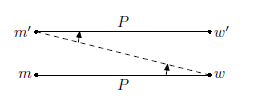
\includegraphics[width=0.4\textwidth]{optimality.png}
  \caption{proof of the optimality \cite{coursera}}
\end{figure}

The theorem indicates that the man-oriented algorithm gives the worst solution for women, and the woman-oriented algorithm gives the worst solution for men.
All other solutions are between these two "particular" solutions.

\subsubsection{Finding all stable solutions} \label{all stable solutions}

By Gale-Shapley algorithm and its optimality, it can be proved that stable marriage problem usually has more than one solution including man-oriented and woman-oriented solution. 
However, they may be inappropriate for most of cases in real world, which raises a natural question that: 
is there other stable solutions, or more fair stable matching than one-side oriented solution available? 
Here, an efficient approach given by McVitie and Wilson in \cite{McVitie&Wilson} will be explained.

The main idea of McVitie and Wilson’s method is to keep {\it break} the exist stable pairs to make the outcome more “biased” toward woman-side and find all stable solutions in this process. 
Specifically, this operation consisted with breaking the marriage of a man $m_i$ and force him to propose from the woman followed by his ex-wife in his preference list.
Once the {\it breakmarriage} operation starts, the dynamic of the method is similar to the Gale-Shapley algorithm.
Some differences from Gale-Shapley dynamic is that: 
there is only one unmarried man in the process at the same time and the woman will only accept the man ranks higher than her current spouse in her preference list.
The operation {\it breakmarriage} will be ended either the unlucky man $m_i$ being rejected by all women (i.e., failed in {\it breakmarriage}), or the new stable marriage is achieved.
As unlimited use of operation {\it breakmarriage} would causes duplicates solutions, there are two further restrictions on {\it breakmarriage} operation: \cite{McVitie&Wilson}

\begin{itemize}
  \item Starting at a stable solution obtained by a {\it breakmarriage} operation on man $m_i$, {\it breakmarriage} may only be performed on man $m_j$ with $i \leq j$
  \item Only man $m_j$ with $i \leq j$ may propose if {\it breakmarriage} is started from man $m_i$.
\end{itemize}

With the conditions and restrictions mentioned above, it can be proved that all stable solutions can be founded.

\begin{theorem}
  (stability)
  Based on a set of stable marriage, the solution provided by successfully breakmarriage operation is stable. \cite{McVitie&Wilson}
\end{theorem}

\paragraph{Proof of stability:} All unaffected pairs are stable since they were stable in previous matching.
If the {\it breakmarriage} operation affects man $m_i$ and finally he get married with woman $w_i$, and if man $m_i$ actually prefers woman $w_j$ than woman $w_i$,
man $m_i$ must had porposed to woman $w_j$ and been rejected by woman $w_j$.
This indicates that woman $w_j$ must prefer her current husband $m_j$.
So the marriage is stable. (end of proof)\\

And with the similar reasoning, it can be shown that\cite{physicist}:

\begin{theorem}
  (accessibility)
  All stable solutions, other than the man-oriented stable solution, can be obtained from the man-oriented stable solution by successive applications of the breakmarriage operations. \cite{McVitie&Wilson}
\end{theorem}

This method is running with a time complexity of $O(n^3 \lvert S \rvert)$, where $S$ is the set of stable marriages \cite{physicist}.
The method will be discussed later in section \ref{performance_analysis}.

\subsection{Assignment problem and Hungarian algorithm} \label{hungarian}

In this subsection, the Hungarian algorithm, or Kuhn-Munkres algorithm, will be introduced to solve the assignment problem,
which can be seen as the same structure with the stable marriage problem when looking for the optimal solution.

\subsubsection{Assignment problem and stable marriage} \label{assignment problem}

The Hungarian method is a combinatorial optimization algorithm capable of solving assignment problems in polynomial time. 
It was firstly developed and proposed by Harold Kuhn in 1955 \cite{Kuhn1955}, 
and was named as "Hungarian method" due to the theoretical basis of previous Hungarian mathematicians: Denes K$\ddot{o}$nig (K$\ddot{o}$nig theorem) and Jeno Egervary.

The assignment problem can be defined as follow: there are $n$ workers $w$ and $n$ assignments $a$.
Each of the workers $w_i$ have different time to finish the corresponding job $a_i$.
The problem aims at finding a one-to-one matching that minimise the total time.
A simple example for the assignment problem is given as follow:
\begin{table}[H]
  \centering
  \begin{tabular}{|c|c|c|c|c|}
    \hline
    Assignment & $w_1$ & $w_2$ & $w_3$ & $w_4$ \\
    \hline
    \hline
    $a_1$ & 90 & 75 & 75 & 80 \\
    \hline
    $a_2$ & 35 & 85 & 55 & 65 \\
    \hline
    $a_3$ & 125 & 95 & 90 & 105 \\
    \hline
    $a_4$ & 45 & 110 & 95 & 115 \\
    \hline
  \end{tabular}
  \caption{An example with costing time matrix for different assignment}
\end{table}

It can be seen that the assignment problem not completely same as the stable marriage problem: it is a 1-sided preference matching rather than two side in traditional stable marriage problem.
But this can be easily to rewrite to the stable marriage problem by changing the certain cost $S_{ij}$ in to the sum of the man's ranking order $x_i$ and woman's ranking order $y_j$.
The certain cost $S_{ij}$ can be seen as the {\it cost} of the matching. The optimal matching can be calculated by minimise the cost $S_{ij} = x_i + y_j$.

\begin{table}[H]
  \centering
  \begin{tabular}{|c|c|c|c|}
    \hline
    Man & Preference list & Woman & Preference list \\
    \hline
    \hline
    $m_1$ & $(w_2, w_4, w_1, w_3)$ & $w_1$ & $(m_2, m_1, m_4, m_3)$ \\
    \hline
    $m_2$ & $(w_3, w_1, w_4, w_2)$ & $w_2$ & $(m_4, m_3, m_1, m_2)$ \\
    \hline
    $m_3$ & $(w_2, w_3, w_1, w_4)$ & $w_3$ & $(m_1, m_4, m_3, m_2)$ \\
    \hline
    $m_4$ & $(w_4, w_1, w_3, w_2)$ & $w_4$ & $(m_2, m_1, m_4, m_3)$ \\
    \hline
  \end{tabular}
\end{table}
\begin{center}
  $\downarrow$
\end{center}  
\begin{table}[H]
  \centering  
    \begin{tabular}{|c|c|c|c|c|}
    \hline
    Cost & $w_1$ & $w_2$ & $w_3$ & $w_4$ \\
    \hline
    \hline
    $m_1$ & 2+1=3 & 0+2=2 & 3+0=3 & 1+1=2 \\
    \hline
    $m_2$ & 1+0=1 & 3+3=6 & 0+3=3 & 2+0=2 \\
    \hline
    $m_3$ & 2+3=5 & 0+1=1 & 1+2=3 & 3+3=6 \\
    \hline
    $m_4$ & 1+2=3 & 3+0=5 & 2+1=3 & 0+2=2 \\
    \hline
  \end{tabular} 
  \caption{Example: transfer preference lists into cost matrix}
\end{table}

\subsubsection{The Hungarian algorithm}

After converting two-sided preferences to cost matrix, the Hungarian algorithm can be used to solve the stable marriage problem.
The basic logic of the Hungarian algorithm is to swap the matching pair and the unmatched vertex in the Augmenting path by looking for the augmenting path until the augmenting path cannot be found.
The algorithm follows these specific steps:

\begin{algorithm}[H]
  \SetAlgoLined
  Begin with the cost matrix\;
  \For{row in cost matrix}{
    Subtract the minimum in each row from every number
  }
  \For{column in cost matrix}{
    Subtract the minimum in each column from every number
  }
  Determine the minimum number $n$ of lines needed to cross out all zeros in the current table\;
  \If{$n$ equals length of matrix}{
    The optimal solution is obtained}
  \Else{
    Subtract the smallest uncrossed number from every uncrossed number and add the smallest uncrossed number to the numbers at intersections of crossing lines}
\end{algorithm}

The code is also available in appendix \ref{GS_algorithm}. 
By K$\ddot{o}$nig theorem, it can be easy to find a minimum set of crossing lines covers all zeros and therefore a maximum set of indepedent zeros.
Hence the optimal solution can be got \cite{Kuhn1955}.
The algorithm is expected to give a minimised cost solution with a time complexity of $O(n^3)$.
However, there is no guarantee on giving a stable solution. 

\section{Experimental and performance analysis} \label{performance_analysis}

In this subsection, algorithms will be finished with python code. 
After running the code, qualitative and quantitative analysis will be performed and gives a general conclusion on the algorithms.

\subsection{Algorithms analysis}

After confirming that the program meets its condition and produces the required results, the outcomes were plotted to make a comparison.

To test two algorithms, there will be 1 to 500 bipartite matching problem random generated and they will be solved by two algorithms.
To compare the time complexity of the results, the running time of algorithms will be recorded. 
Also, as the matching outcome may not direct, the cost for the matching and the amount of unstable pairs will be involved to give a relatively direct comparison. 

\subsubsection{Comparison on two algorithms:} 
The outcome given by two different algorithms are presented as follow: 

\begin{figure}[H]
  \centering
  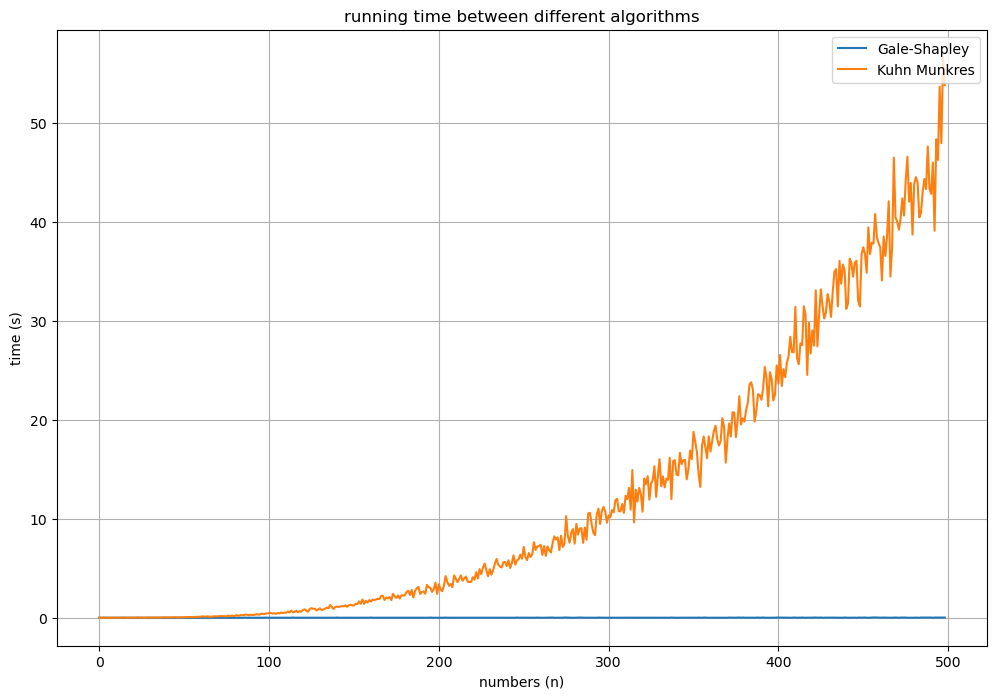
\includegraphics[width=0.6\textwidth]{running_time_2_algorithms.png}
  \caption{Duration between two algorithms.}
\end{figure} 

It can be seen that compared with Kuhn-Munkres, the time consumption of Gale-Shapley algorithm keeps in a very low level. 
It is running with the time complexity of $O(n^2)$ while Kuhn-Munkres is running with the time complexity of $O(n^3)$.

\begin{figure}[H]
  \centering
  \subfigure[Percentage of unstable pairs in Kuhn-Munkres]{
    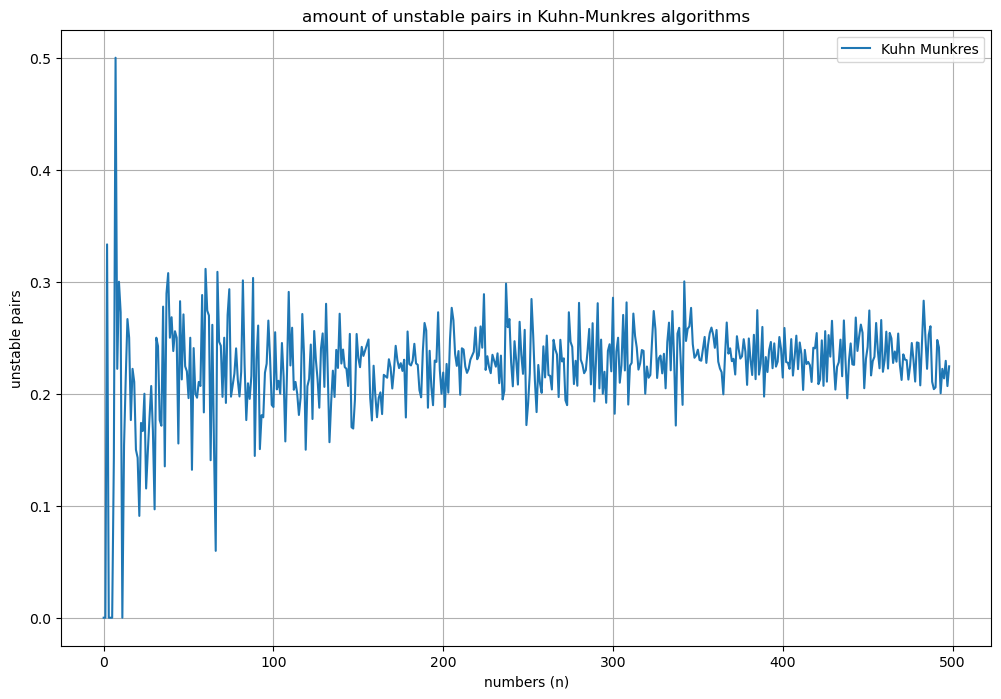
\includegraphics[width=0.45\textwidth]{percentage_of_unstable_pairs_in_KM.png}
  } 
  \quad
  \subfigure[Cost between two algorithms]{
    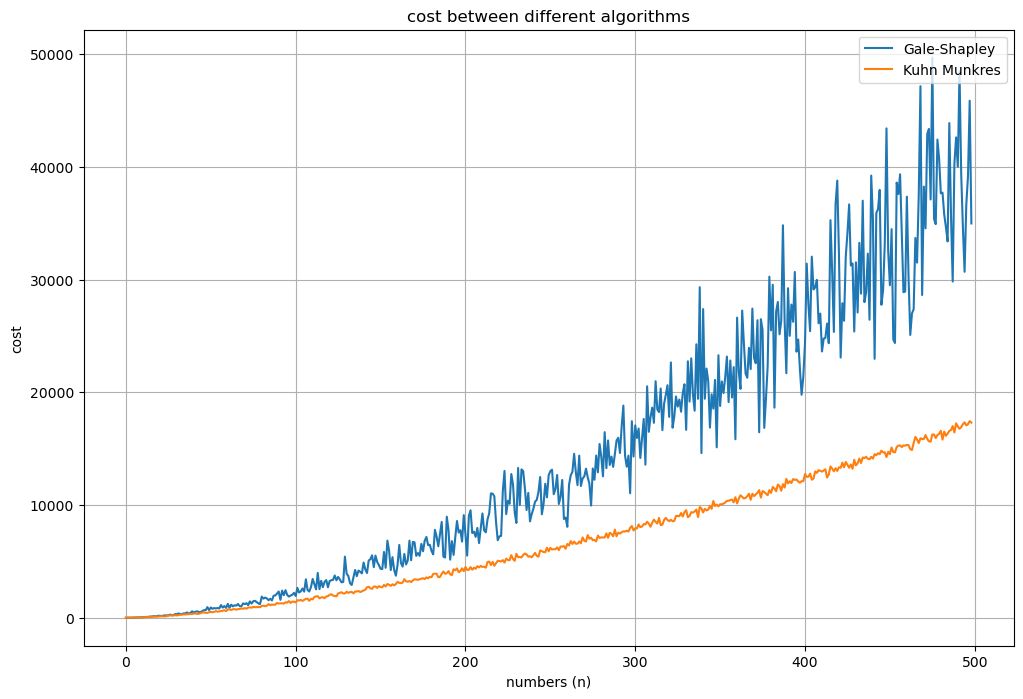
\includegraphics[width=0.45\textwidth]{cost_2_algorithms.png}
  }    
  \caption{Outcome analysis between two algorithms}
\end{figure}

In terms of unstable pairs, it can be seen that majority of pairs are stable.
With $n$ growth, there are still 25\% of the pairs are unstable in the outcome given by Kuhn-Munkres algorithm.
While in terms of cost, Kuhn-Munkres provided an approach with a lower cost and less volatility than Gale-Shapley.
As Kuhn-Munkres gives a global optimal solution and Gale-Shapley gives a individual stability solution, this may causes a tradeoff between two algorithms in pratical applications.

\subsubsection{Unfairness on Gale-Shapley:} 
The unfairness of Gale-Shapley algorithm is also tested as follow: \label{unfair_GS}

\begin{figure}[H]
  \centering
  \subfigure[Cost difference in man-oriented GS algorithm]{
    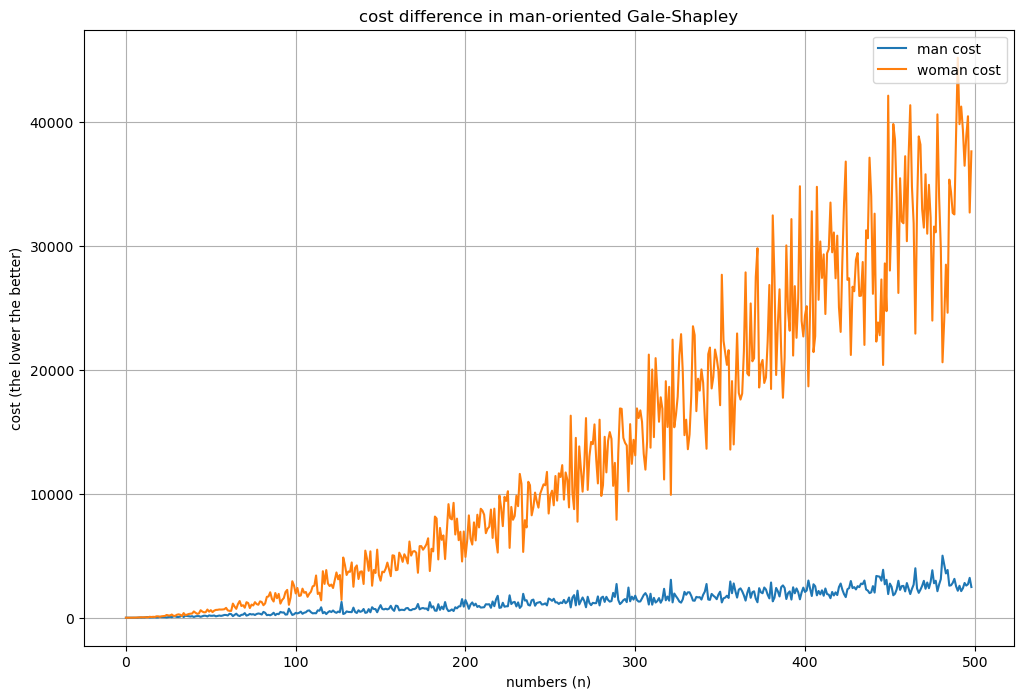
\includegraphics[width=0.45\textwidth]{cost_in_man_oriented_in_GS.png}
  }   
  \quad
  \subfigure[Percentage of same solution]{
    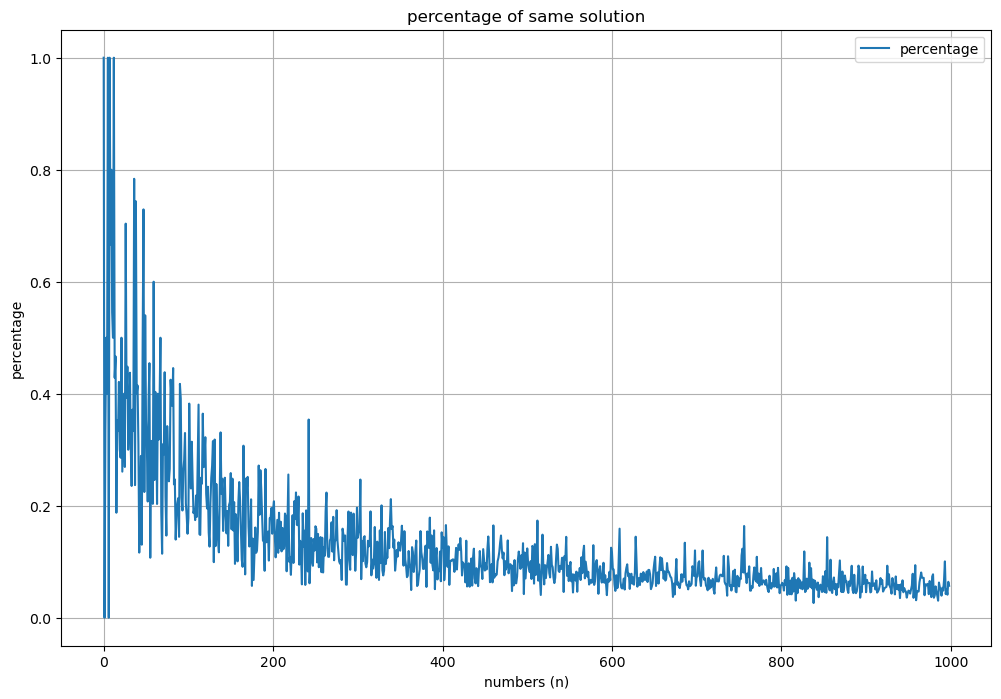
\includegraphics[width=0.45\textwidth]{percentage of same solution.png}
  } 
  \caption{Unfairness in man-oriented Gale-Shapley algorithm}
\end{figure}

It can be seen that in man-oriented Gale-Shapley algorithm (graph (a)), there is a noticeable difference in cost between man and woman.
It is obvious that the algorithm is unfair to the woman side, woman cost several times more than man in the same matching. (There is no claim about real life)

Also, there is a comparison on the same pairs between man-oriented algorithm and woman-oriented algorithm (graph (b)).
It can be seen that as $n$ increase, the percentage of same solution given by different oriented algorithm converge to approximately below 10\%,
which might indicate that in man-oriented Gale-Shapley algorithm, there is only very small proportion of women candidates can get same result as it in woman-oriented algorithm.

Besides, as all stable matching can be got by {\it breakmarriage} operations (mentioned in subsection \ref{all stable solutions}), 
the dynamic of cost changing in {\it breakmarriage} operations is also presented as follow:

\begin{figure}[H]
  \centering
  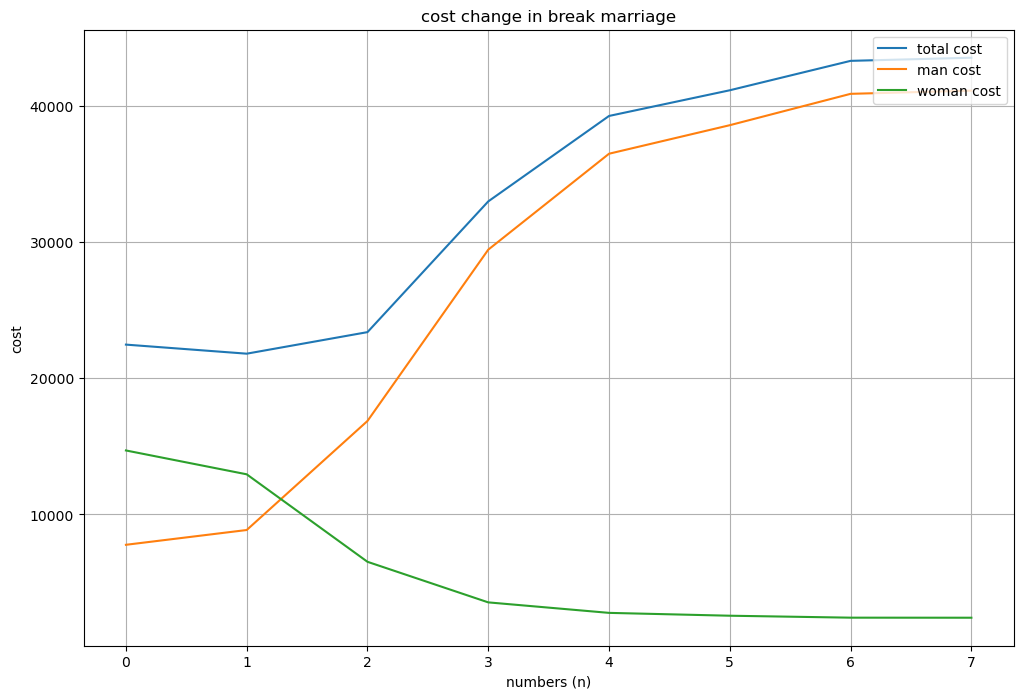
\includegraphics[width=0.6\textwidth]{cost change in breakmarriage.png}
  \caption{Cost change in {\it breakmarriage} operations.}
\end{figure} 

Here, there are 8 stable matchings generated by the {\it breakmarriage} operations from a 500-500 matching problem (man-oriented solution is not included).
It can be seen that with $n$ increases, the cost of "man-side" increases while the cost of "woman-side" decreases.
The minimum total cost appears near to the intersection of man-cost curve and woman-cost curve.

\subsection{Trials on improvement} 

After comparing between two different algorithms, it can be found that the stability, total cost and time complexity forms an "impossible triangle".
But it is possible to make improvements on two algorithms.

\subsubsection{Improvement on Gale-Shapley}

As mentioned last subsection, the minimum of total cost appears nears to the intersection of man-cost and woman-cost curve in the process of {\it breakmarriage} operations. 
So, by going through every stable matching, the balanced solution with less cost and balanced stable matching can be used as a solution.
The code is available in appendix \ref{GS_algorithm}.

\begin{figure}[H]
  \centering
  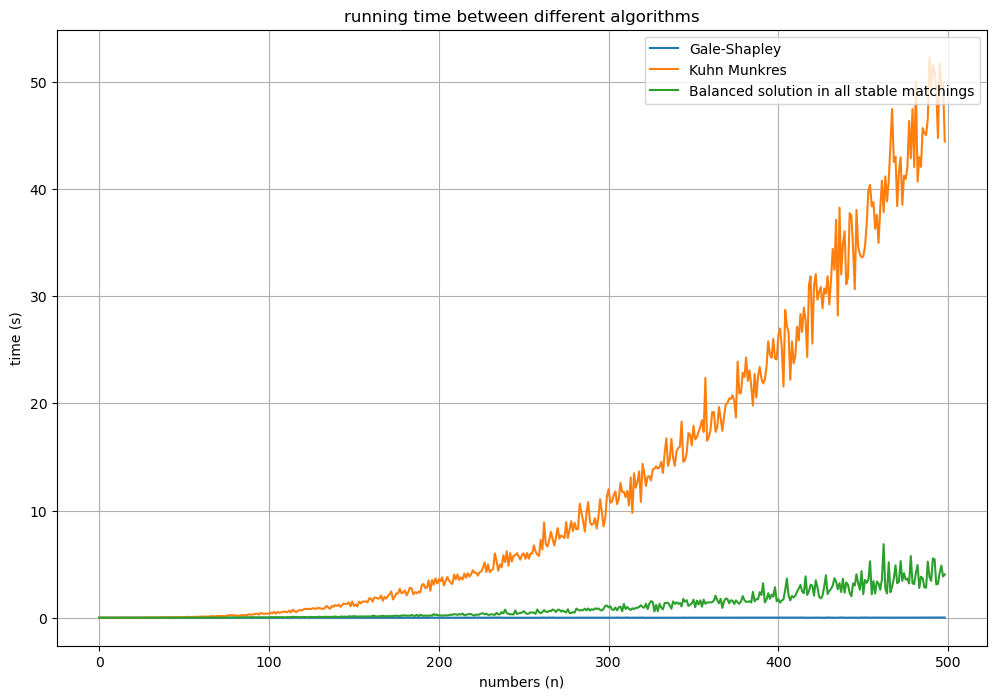
\includegraphics[width=0.6\textwidth]{running time all.png}
  \caption{Durations of 3 algorithms.}
\end{figure}

In time complexity analysis, it can be seen that although the new method takes much more time than original Gale-Shapley algorithm, it still has a great advantage over Kuhn-Munkres.

\begin{figure}[H]
  \centering
  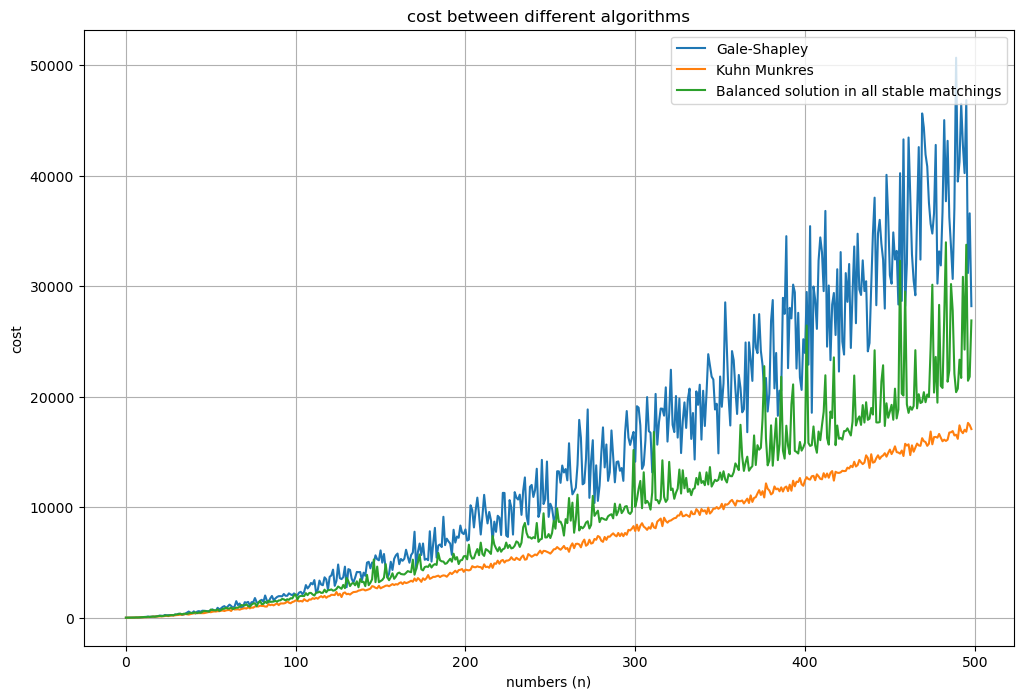
\includegraphics[width=0.6\textwidth]{cost all.png}
  \caption{Cost of 3 algorithms.}
\end{figure}

And in terms of outcome analysis, as all the pairs are stable, only cost differences are presented. 
The new method effectively reduces the cost of Gale-Shapley algorithm and have about 20\% more cost than Kuhn-Munkres.

In summary, the new method provides a choice with a relatively lower cost and balanced solution. 
Although it might meaningless in solving the problem of marriage (as it is not realistic to only allow some of women break the marriage but others cannot), it may gives another choice and may be useful in some other area.

\subsubsection{Improvement on Kuhn-Munkres}

As Kuhn-Munkres takes several times more than Gale-Shapley, a natural idea is that there may be a method to combine the advantage of two algorithms.

Here a combination between two algorithms was considered. 
As Gale-Shapley takes very few time than Kuhn-Munkres, it may possible to reduce the running time of Kuhn-Munkres by firstly carry out Gale-Shapley.
Specifically, there are about 10\% of same solution conducted by man-oriented and woman-oriented Gale-Shapley algorithm (mentioned in \ref{unfair_GS}). 
As the Kuhn-Munkres is running with a time complexity of $O(n^3)$, there is expected to reduce the time with a similar cost.

So, the method named as "mixed" was written and tested. 
The basic idea is firstly running man-oriented Gale-Shapley and woman-oriented Gale-shapley, removes candidates with the same solutions, 
then carry out Kuhn-Munkres with the rest of candidates.
The code is available in appendix \ref{GS_algorithm}.

The outcome given by new method are presented as follow:

\begin{figure}[H]
  \centering
  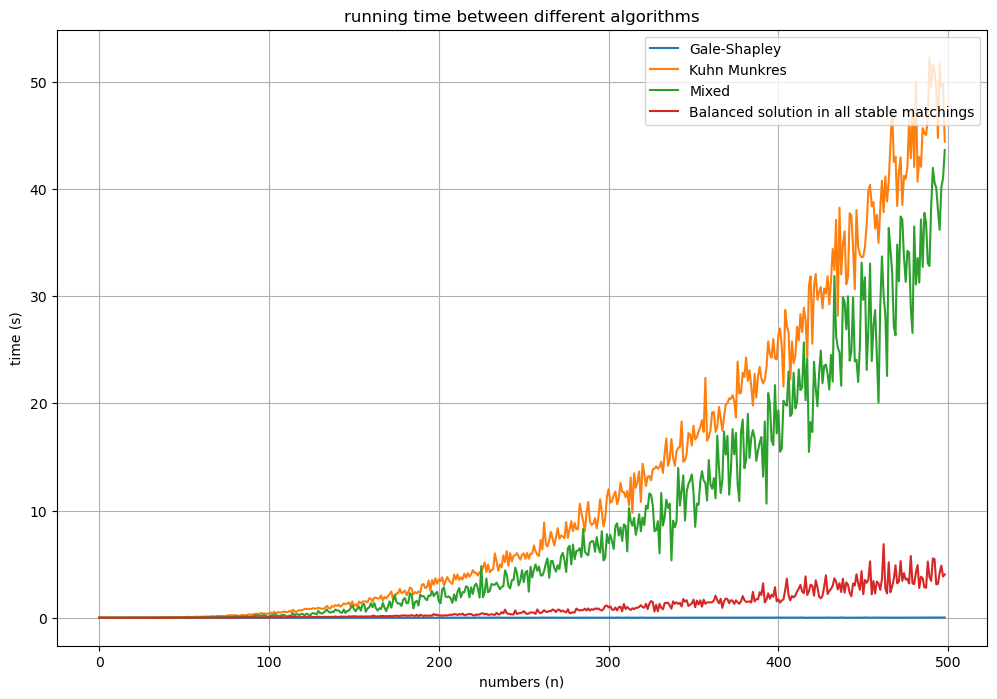
\includegraphics[width=0.6\textwidth]{running time mixed all.png}
  \caption{Durations of 3 algorithms.}
\end{figure} 

As expected, compared to Kuhn-Munkres, there is a noticeable reduction on time. 
Because Kuhn-Munkres has a time complexity of $O(n^3)$, approximately 20\% of the time was saved.
But it still takes much more time than Gale-Shapley algorithm.

\begin{figure}[H]
  \centering
  \subfigure[Unstable pairs]{
    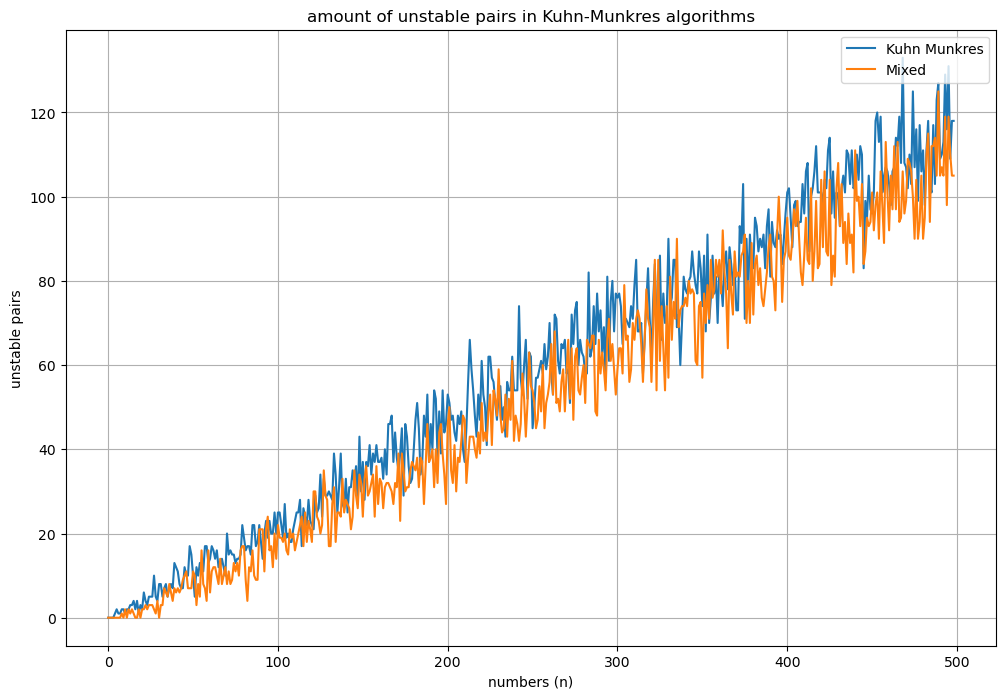
\includegraphics[width=0.45\textwidth]{unstable_pairs_mixed.png}
  }   
  \quad
  \subfigure[Cost of 3 algorithms]{
    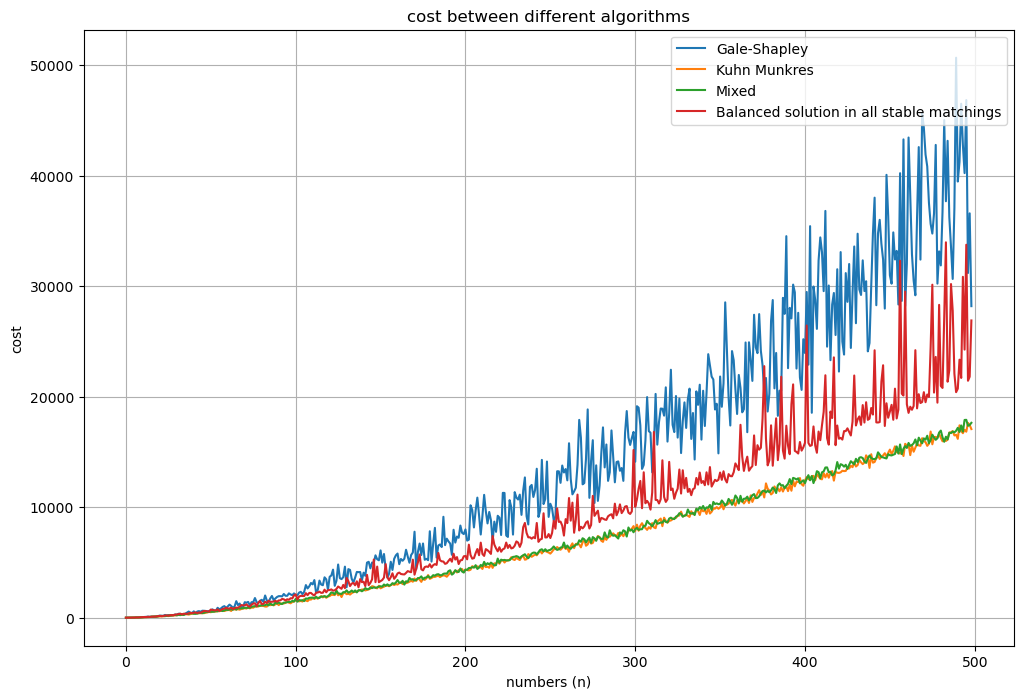
\includegraphics[width=0.45\textwidth]{cost mixed all.png}
  } 
  \caption{Outcome analysis for 3 algorithms}
\end{figure}

Also, in terms of stability, the new method conducts relatively less unstable pairs than Kuhn-Munkres algorithm in maority of time.
Besides, in terms of cost, the new method keeps a same level with Kuhn-Munkres algorithm, which is significantly less than Gale-Shapley algorithm.

\begin{figure}[H]
  \centering
  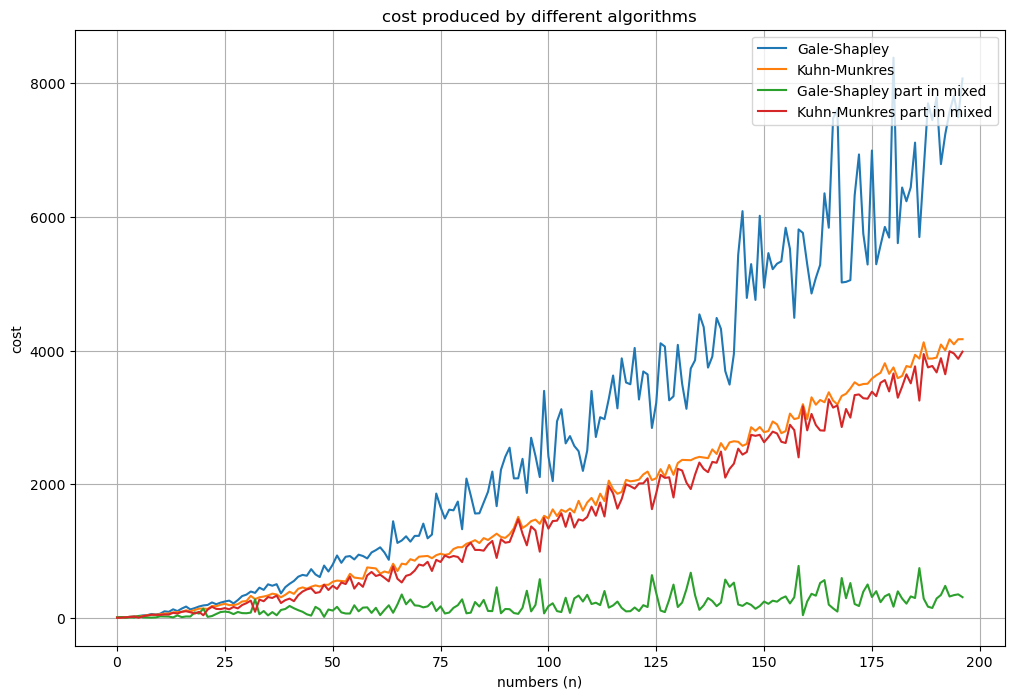
\includegraphics[width=0.6\textwidth]{cost_produced_by_different_algorithms.png}
  \caption{Cost produced by different components.}
\end{figure} 

Specifically, by analyzing on different parts of the new method, 
it can be seen that majority of cost are contributed by Kuhn-Munkres part, which makes sense since majority pairs are Kuhn-Munkres pair.
Also, as the amount of Gale-Shapley pairs is limited, the Gale-Shapley part does not contribute much.
It only slightly raises the total cost than traditional Kuhn-Munkres.

In summary, the new method reduces approximately 20\% of the running time and keeps the cost with the same level of Kuhn-Munkres.
This might be meaningful when $n$ becomes sufficient large.

\section{Conclusion and discussion}

In this report, stable marriage problem and its algorithms were focused. 
The primary conceptions about matching in graph and stable marriage problem were firstly given to construct the theoretical basis, together with two primary goals, individual stable and global optimal, in this research.
After that, two widely-used algorithms, including Gale-Shapley and Hungarian, with different stress on primary goals, are introduced to solve the stable marriage problem.
The method of finding all stable matching based on Gale-Shapley dynamic, together with some related theorems and facts are also being introduced and proved.
Finally, the performance analysis was performed to give a direct comparison on time complexity and accuracy. 
In this part, the cost and unstable pairs are involved to measure the accuracy. Python programs were finished to give a quantitative comparison. 
And the outcomes were plotted to give a qualitative conclusion.
It can be found that Gale-Shapley gives stable solutions while Hungarian gives global optimal solutions.
Some trials of improvements are also being performed and tested with two algorithms mentioned above. 
By iterating through all the stable solution, the balanced stable solution was generated to reduce the overall cost given by traditional Gale-Shapley algorithm.
By combined the advantage of two algorithms, an improvement was made to reduce the running time of the Hungarian algorithm.

Although there has been lots of contents covered by the project, there are still some compromises in this project. Some points still require further discussion and analysis, mainly including following parts:
\begin{itemize}
  \item This project mainly focused on traditional algorithms. However, many heuristic algorithms such as ant colony and ANN could give better outcome than traditional algorithms.
  \item The project only focus on stable marriage problem with complete lists. This model can only covers a very small part of problems in real life. The incomplete perference problem, together with other variants, are also worthing further research.
  \item There are also still many variants of Gale-Shapley and Hungarian algorithm. This report cannot cover all of them and gives detailed investigations.
\end{itemize}

\section*{Acknowledgement}

The author would like to express the appreciation to the supervisor of the project Dr. Aistis Atminas, who support this work with supportive material, academic and technical advice and enlightenment.
and Lin Jiao, Muxun Zhao and Ziyu Zhou who helped in finding the logical loopholes and providing supports on the project.

\newpage
\section*{Appendix: Python code} \label{GS_algorithm}
\begin{python} 
import copy
import matplotlib.pyplot as plt
import numpy as np
import random
import scipy
import time

from munkres import Munkres, print_matrix

#######################################################################
############################# main method #############################
#######################################################################

def main():
    
    # automated test
    n = 500
    [preference_matrix_list_gs, outcome_list_gs, duration_list_gs, cost_gs, unstable_pairs_list_gs, unstable_percentage_list_gs] = automated_test(n, 'gs')
    [preference_matrix_list_km, outcome_list_km, duration_list_km, cost_km, unstable_pairs_list_km, unstable_percentage_list_km] = automated_test(n, 'km')
    [preference_matrix_list_mixed, outcome_list_mixed, duration_list_mixed, cost_mixed, unstable_pairs_list_mixed, unstable_percentage_list_mixed] = automated_test(n, 'mixed')
    [preference_matrix_list_all, outcome_list_all, duration_list_all, cost_all, unstable_pairs_list_all, unstable_percentage_list_all] = automated_test(n, 'all_stable_matching')

    ############################# GS & KM #############################

    # plot duration 
    plt.figure(figsize=(12,8))
    plt.plot(duration_list_gs, label='Gale-Shapley')
    plt.plot(duration_list_km, label='Kuhn Munkres')
    plt.grid(True)
    plt.xlabel('numbers (n)')
    plt.ylabel('time (s)')
    plt.legend(loc='upper right')
    plt.title('running time between different algorithms') 

    # plot total cost
    plt.figure(figsize=(12,8))
    plt.plot(cost_gs, label='Gale-Shapley')
    plt.plot(cost_km, label='Kuhn Munkres')
    plt.grid(True)
    plt.xlabel('numbers (n)')
    plt.ylabel('cost')
    plt.legend(loc='upper right')
    plt.title('cost between different algorithms')  

    # plot the amount of unstable pairs
    plt.figure(figsize=(12,8))
    plt.plot(unstable_pairs_list_km, label='Kuhn Munkres')
    plt.grid(True)
    plt.xlabel('numbers (n)')
    plt.ylabel('unstable pairs')
    plt.legend(loc='upper right')
    plt.title('amount of unstable pairs in Kuhn-Munkres algorithms') 

    # plot the percentage of unstable pairs
    plt.figure(figsize=(12,8))
    plt.plot(unstable_percentage_list_km, label='Kuhn Munkres')
    plt.grid(True)
    plt.xlabel('numbers (n)')
    plt.ylabel('unstable pairs')
    plt.legend(loc='upper right')
    plt.title('amount of unstable pairs in Kuhn-Munkres algorithms') 
    
    ############################### mixed ###############################

    # plot duration 
    plt.figure(figsize=(12,8))
    plt.plot(duration_list_gs, label='Gale-Shapley')
    plt.plot(duration_list_km, label='Kuhn Munkres')
    plt.plot(duration_list_mixed, label='Mixed')
    plt.grid(True)
    plt.xlabel('numbers (n)')
    plt.ylabel('time (s)')
    plt.legend(loc='upper right')
    plt.title('running time between different algorithms') 

    # plot total cost
    plt.figure(figsize=(12,8))
    plt.plot(cost_gs, label='Gale-Shapley')
    plt.plot(cost_km, label='Kuhn Munkres')
    plt.plot(cost_mixed, label='Mixed')
    plt.grid(True)
    plt.xlabel('numbers (n)')
    plt.ylabel('cost')
    plt.legend(loc='upper right')
    plt.title('cost between different algorithms')  

    # plot the amount of unstable pairs
    plt.figure(figsize=(12,8))
    plt.plot(unstable_pairs_list_km, label='Kuhn Munkres')
    plt.plot(unstable_pairs_list_mixed, label='Mixed')
    plt.grid(True)
    plt.xlabel('numbers (n)')
    plt.ylabel('unstable pairs')
    plt.legend(loc='upper right')
    plt.title('amount of unstable pairs in Kuhn-Munkres algorithms') 
    
    ################################ all ################################
    
    # plot duration 
    plt.figure(figsize=(12,8))
    plt.plot(duration_list_gs, label='Gale-Shapley')
    plt.plot(duration_list_km, label='Kuhn Munkres')
    plt.plot(duration_list_all, label='Balanced solution in all stable matchings')
    plt.grid(True)
    plt.xlabel('numbers (n)')
    plt.ylabel('time (s)')
    plt.legend(loc='upper right')
    plt.title('running time between different algorithms') 

    # plot duration 
    plt.figure(figsize=(12,8))
    plt.plot(duration_list_gs, label='Gale-Shapley')
    plt.plot(duration_list_km, label='Kuhn Munkres')
    plt.plot(duration_list_mixed, label='Mixed')
    plt.plot(duration_list_all, label='Balanced solution in all stable matchings')
    plt.grid(True)
    plt.xlabel('numbers (n)')
    plt.ylabel('time (s)')
    plt.legend(loc='upper right')
    plt.title('running time between different algorithms') 

    # plot total cost
    plt.figure(figsize=(12,8))
    plt.plot(cost_gs, label='Gale-Shapley')
    plt.plot(cost_km, label='Kuhn Munkres')
    plt.plot(cost_all, label='Balanced solution in all stable matchings')
    plt.grid(True)
    plt.xlabel('numbers (n)')
    plt.ylabel('cost')
    plt.legend(loc='upper right')
    plt.title('cost between different algorithms') 

    # plot total cost
    plt.figure(figsize=(12,8))
    plt.plot(cost_gs, label='Gale-Shapley')
    plt.plot(cost_km, label='Kuhn Munkres')
    plt.plot(cost_mixed, label='Mixed')
    plt.plot(cost_all, label='Balanced solution in all stable matchings')
    plt.grid(True)
    plt.xlabel('numbers (n)')
    plt.ylabel('cost')
    plt.legend(loc='upper right')
    plt.title('cost between different algorithms') 

#######################################################################
############################# algorithms ##############################
#######################################################################

######################## Gale Shapley algorithm #######################

def gale_shapley(n, menPreferences, womenPreferences, default = "Not") -> list:
    '''
    the main body of Gale Shapley algorithm
    :param n: int, the length of menPreferences and womenPreferences
    :param menPreferences: list of list, store the preference for each man
    :param womenPreferences: list of list, store the preference for each women
    :return: list, return men's spouse
    '''
    n = len(menPreferences)
    unmarriedMen = list(range(n))
    manSpouse = [None] * n
    womanSpouse = [None] * n
    nextManChoice = [0] * n
    # While there exists at least one unmarried man:
    while unmarriedMen:
        he = unmarriedMen[0]
        hisPreferences = menPreferences[he]
        she = hisPreferences[nextManChoice[he]]
        herPreferences = womenPreferences[she]
        currentHusband = womanSpouse[she]
        if currentHusband is None:
            manSpouse[he] = she
            womanSpouse[she] = he
            unmarriedMen.remove(he)
            nextManChoice[he] += 1
        else:
            if herPreferences.index(he) < herPreferences.index(currentHusband):
                manSpouse[he] = she
                womanSpouse[she] = he
                unmarriedMen.remove(he)
                nextManChoice[he] += 1
                unmarriedMen.append(currentHusband)
            else:
                nextManChoice[he] += 1
                continue
    # printer        
    if default == "print":
        print("the outcome of Gale Shapley algorithm is:")
        i = 0
        for man in manSpouse:
            print(f'man {i+1} -> woman {man+1}')
            i += 1
    return manSpouse

def gale_shapley_with_breakmarriage(n, menPreferences, womenPreferences, manSpouse, dumped_man) -> list:
    '''
    the main body of Gale Shapley algorithm
    :param n: int, the length of menPreferences and womenPreferences
    :param menPreferences: list of list, store the preference for each man
    :param womenPreferences: list of list, store the preference for each women
    :param manSpouse: list, store the current wife for each man
    :param dumped_man: int, the man being damped by his spouse
    :return: list, return men's spouse
    '''
    # initial setup
    unmarriedMen = list()
    unmarriedMen.append(dumped_man)    
    newWomanSpouse = [None] * n
    womanSpouse = [None] * n
    for man in range(len(newWomanSpouse)):
        woman = manSpouse[man]        
        womanSpouse[woman] = copy.copy(man)
        if man != dumped_man:
            newWomanSpouse[woman] = man 
    nextManChoice = [0] * n
    nextManChoice[dumped_man] = menPreferences[dumped_man].index(manSpouse[dumped_man]) + 1
    # While there exists at least one unmarried man:
    while unmarriedMen: 
        he = unmarriedMen[0]
        # Examine if there is out of index    
        if nextManChoice[he] >= n:
            manSpouse = "the breakmarriage failed"
            break 
        hisPreferences = menPreferences[he]
        she = hisPreferences[nextManChoice[he]]
        herPreferences = womenPreferences[she]
        # she only accpet better choice
        if herPreferences.index(he) > herPreferences.index(womanSpouse[she]):
            nextManChoice[he] += 1
            continue 
        currentHusband = newWomanSpouse[she]
        # If she have no spouse        
        if currentHusband is None:
            manSpouse[he] = she
            newWomanSpouse[she] = he
            unmarriedMen.remove(he)
            nextManChoice[he] += 1 
        # If she have a spouse    
        else:
            if herPreferences.index(he) < herPreferences.index(currentHusband):
                manSpouse[he] = she
                newWomanSpouse[she] = he
                unmarriedMen.remove(he)
                nextManChoice[he] += 1
                unmarriedMen.append(currentHusband)
                continue
            else:
                nextManChoice[he] += 1
                continue  
    return manSpouse

######################## Kuhn-Munkres algorithm #######################

def kuhn_munkres(cost_matrix, print_status = "Not") -> list:
    '''
    the main body of Kuhn Munkres algorithm, or Hungarian algorithm
    :param cost_matrix: n * n list, cost matrix generated by the def matrix_converter(n, menPreferences, womenPreferences, default = "cost")
    :param print_status: String, default == "Not", input "print_all" to print the outcome
    :return: list, return men's spouse
    '''
    print(f'km n = {len(cost_matrix)}')
    # make a copy of cost matrix
    matrix = matrix_deep_copy(cost_matrix)
    # start running
    m = Munkres()
    indexes = m.compute(matrix)
    manSpouse = list()
    # transfer indexes tuple into manSpouse list
    for row, column in indexes:
        manSpouse.append(column)
    # printer    
    if print_status == "print_all":
        print_matrix(matrix, msg="Lowest cost through this matrix:")
        total_cost = 0
        print("the outcome of Kuhn-Munkres algorithm is:")
        for row, column in indexes:
            print(f'man {row+1} -> woman {column+1} (with the cost of {cost_matrix[row][column]})')
            total_cost += cost_matrix[row][column]
        print(f'the total cost is {total_cost}')    
    elif print_status == "print":
        print("the outcome of Kuhn-Munkres algorithm is:")
        for row, column in indexes:
            print(f'man {row+1} -> woman {column+1}')      
    return manSpouse

########################### Mixed algorithm ###########################

def mixed_algorithm(n, menPreferences, womenPreferences, default = "default") -> list:
    '''
    the main body of a kind of mixed algorithm
    The optimal solution given by man-oriented and woman-oriented gs algorithm will be given
    And rest of parts will perform Hungarian to get a lower cost
    :param n: int, the length of menPreferences and womenPreferences
    :param menPreferences: list of list, store the preference for each man
    :param womenPreferences: list of list, store the preference for each women
    :return: list, return men's spouse
    '''
    print(f'mixed n = {n}')
    # initial setup
    result = list()
    for i in range(n):
        result.append(-1)
    index = list(range(n)) # mapping km candidate into whole list
    result_type = list() # algorithm used to solve the problem
    for i in range(n):
        result_type.append(-1) # -1 for km and 1 for gs
    # get copies for menPreferences and womenPreferences
    menPreferences_copy = matrix_deep_copy(menPreferences)
    womenPreferences_copy =  matrix_deep_copy(womenPreferences)   
    # get optimal choice by man-oriented gs and woman-oriented gs
    men_outcome = manSpouse_to_dict(gale_shapley(n, menPreferences_copy, womenPreferences_copy))
    women_outcome_unchanged = manSpouse_to_dict(gale_shapley(n, womenPreferences_copy, menPreferences_copy))
    women_outcome = resort_dict(change_key_to_value(women_outcome_unchanged))
    # get simplified preferences lists 
    simplified_menPreferences = matrix_deep_copy(menPreferences_copy)
    simplified_womenPreferences = matrix_deep_copy(womenPreferences_copy)
    # input optimal pairs given by gs algorithm into result list and remove them from the preferences list
    counter = 0
    for man in range(len(men_outcome)):
        if men_outcome[man] == women_outcome[man]:
            # the optimal pair
            woman = men_outcome[man]
            # input the result
            result[man] = woman
            # remove the man from woman's preference list
            for i in range(len(simplified_womenPreferences)):
                simplified_womenPreferences[i].remove(man)
            for i in range(len(womenPreferences_copy)):
                womenPreferences_copy[i].remove(man)
            simplified_womenPreferences.remove(womenPreferences_copy[woman]) 
            # remove the woman from man's preference list
            for i in range(len(simplified_menPreferences)):
                simplified_menPreferences[i].remove(woman)   
            for i in range(len(menPreferences_copy)):
                menPreferences_copy[i].remove(woman) 
            simplified_menPreferences.remove(menPreferences_copy[man]) 
            # remove paired women from index list    
            index.remove(woman) 
            result_type[man] = 1 
            counter += 1        
    # check if there exists unmatched pair   
    if -1 in result:            
        # carry out the Hungarian algorithm by using simplified preference list
        cost_matrix = matrix_converter(len(simplified_menPreferences), simplified_menPreferences, simplified_womenPreferences, False)
        km_outcome = kuhn_munkres(cost_matrix)
        # input the Hungarian outcome into result
        number = 0
        for man in range(n):
            if result_type[man] == -1: # Hungarian
                result[man] = index[km_outcome[number]]
                number += 1
    if default == "type_also":            
        return result, result_type      
    else:
        return result  

######################## all stable matchings #########################
 
def all_stable_GS(n, menPreferences, womenPreferences) -> list:
    # initial setup
    man_oriented = gale_shapley(n, menPreferences, womenPreferences)
    all_stable_matchings = list()
    all_stable_matchings.append(man_oriented)
    # start iterate through all possible matchings  
    manSpouse = copy.copy(man_oriented) 
    for man in range(n): 
        dumped_man = copy.copy(man)
        for trial in range(n):
            manSpouse_copy = copy.copy(manSpouse)
            new_matching = gale_shapley_with_breakmarriage(n, menPreferences, womenPreferences, manSpouse_copy, dumped_man)
            if new_matching == "the breakmarriage failed":
                break
            elif new_matching == manSpouse:
                break
            else:
                all_stable_matchings.append(new_matching)
                manSpouse = copy.copy(new_matching)
    return all_stable_matchings 

def balanced_stable_matching(n, menPreferences, womenPreferences) -> list:
    # initial setup
    minimum_cost = None
    balanced_matching = None
    # generate all stable matching
    all_stable_matchings = all_stable_GS(n, menPreferences, womenPreferences)
    # calculate the one side cost matrix    
    man_cost_matrix = one_side_matrix_converter(n, menPreferences, womenPreferences, "man-only")
    woman_cost_matrix = one_side_matrix_converter(n, menPreferences, womenPreferences, "woman-only")
    # iterate through all stable matching
    for matching in all_stable_matchings:
        man_cost = calculate_cost(man_cost_matrix, matching)
        woman_cost = calculate_cost(woman_cost_matrix, matching)
        difference = abs(man_cost - woman_cost)
        if minimum_cost is None:
            minimum_cost = difference
            balanced_matching = matching
        elif minimum_cost > difference:
            minimum_cost = difference
            balanced_matching = matching
        else:
            pass
    return balanced_matching        

#######################################################################
######################### automated testing ###########################
#######################################################################

def automated_test(n, algorithm):
    '''
    the automate test for 3 different algorithms program
    :param n: int, perform 1 to n bipartite matching
    :param algorithm: String, "gs" for Gale-Shapley, "km" for Kuhn-Munkres, "km_percentage" for Kuhn-Munkres with unstable list cosisted with percentage
    :return: list, list consist with [preference_matrix_list, outcome_list, duration_list, cost, unstable_pairs_list]
    '''
    # initial setup
    preference_matrix_list = list()
    outcome_list = list()
    duration_list = list()
    cost = list()
    unstable_pairs_list = list()
    unstable_percentage_list = list()
    # start the test
    for i in range(1, n):        
        # generate the preference list
        menPreferences = generate_random_matrix(i)
        womenPreferences = generate_random_matrix(i)
        # calculate the cost matrix
        cost_matrix = matrix_converter(i, menPreferences, womenPreferences)
        # record the starting time        
        start_time = time.time()
        # Gale-Shapley algorithm    
        if algorithm == "gs":
            outcome = gale_shapley(i, menPreferences, womenPreferences)
            # record the ending time
            end_time = time.time()
            duration = end_time - start_time
            # input the outcome
            preference_matrix = {'menPreferences': menPreferences, 'womenPreferences': womenPreferences}
            preference_matrix_list.append(preference_matrix)
            outcome_list.append(outcome)
            duration_list.append(duration)
            cost.append(calculate_cost(cost_matrix, outcome))
        # Hungarian algorithm    
        elif algorithm == "km":
            outcome = kuhn_munkres(cost_matrix)
            # record the ending time
            end_time = time.time()
            duration = end_time - start_time
            # calculate the unstable pair
            unstable_pair = count_unstable_pair(menPreferences, womenPreferences, outcome)
            # input the outcome
            preference_matrix = {'menPreferences': menPreferences, 'womenPreferences': womenPreferences}
            preference_matrix_list.append(preference_matrix)
            outcome_list.append(outcome)
            duration_list.append(duration)
            cost.append(calculate_cost(cost_matrix, outcome))
            unstable_percentage = unstable_pair / i
            unstable_pairs_list.append(unstable_pair)
            unstable_percentage_list.append(unstable_percentage)
        # mixed algorithm        
        elif algorithm == "mixed": 
            outcome = mixed_algorithm(i, menPreferences, womenPreferences)   
            # record the ending time
            end_time = time.time()
            duration = end_time - start_time
            # calculate the unstable pair
            unstable_pair = count_unstable_pair(menPreferences, womenPreferences, outcome)
            # input the outcome
            preference_matrix = {'menPreferences': menPreferences, 'womenPreferences': womenPreferences}
            preference_matrix_list.append(preference_matrix)
            outcome_list.append(outcome)
            duration_list.append(duration)
            cost.append(calculate_cost(cost_matrix, outcome))
            unstable_percentage = unstable_pair / i
            unstable_pairs_list.append(unstable_pair)
            unstable_percentage_list.append(unstable_percentage)
        # all stable matching 
        elif algorithm == "all_stable_matching":
            outcome = balanced_stable_matching(i, menPreferences, womenPreferences)   
            # record the ending time
            end_time = time.time()
            duration = end_time - start_time
            # input the outcome
            preference_matrix = {'menPreferences': menPreferences, 'womenPreferences': womenPreferences}
            preference_matrix_list.append(preference_matrix)
            outcome_list.append(outcome)
            duration_list.append(duration)
            cost.append(calculate_cost(cost_matrix, outcome))
    return preference_matrix_list, outcome_list, duration_list, cost, unstable_pairs_list, unstable_percentage_list

#######################################################################
######################### supportive methods ##########################
#######################################################################    

# generate random preference matrix

def generate_random_matrix(n) -> list:
    '''
    the method used to generate n * n preference list 
    :param n: int, the amount of person
    :return: list of list, the list for preference lists
    '''
    preference_matrix = list()
    for i in range(n):
        shuffle = random.sample(list(range(n)),n)
        preference_matrix.append(shuffle)
    return preference_matrix

# calculate the cost matrix

def matrix_converter(n, menPreferences, womenPreferences, default = True, type = "cost") -> list:
    '''
    the method used to calculate the cost matrix with two preferences lists, the key step of transfering 2-sided matching into 1-sided matching
    :param n: int, the length of menPreferences and womenPreferences
    :param menPreferences: list of list, store the preference for each man
    :param womenPreferences: list of list, store the preference for each women
    :param default: Boolean, default = True, input False if indexing is needed
    :param type: String, type = "cost", input "profit" to generate the profit matrix
    :return: list of list, the cost (profit) matrix
    '''
    matrix = np.zeros((n,n), dtype = float)
    # reindexing if needed
    if default == False:
        men_index = copy.copy(womenPreferences[0])
        men_index.sort()
        women_index = copy.copy(menPreferences[0])
        women_index.sort()
    # Firstly, input the men preference into the matrix
    # Pick perference list of each man
    for he in range(n):
        hisPreference = menPreferences[he]
        # Pick every person on his preference list
        for j in range(n):
            # Pick the woman's index 
            she = hisPreference[j]   
            # Input the value into matrix
            if default == False:
                herIndex = women_index.index(she)
                matrix[he, herIndex] = j
            else:                 
                matrix[he, she] = j  
    # Secondly, input the women preference into the matrix
    # Pick perference list of each woman
    for she in range(n):
        herPreference = womenPreferences[she]
        # Pick every person on her preference list
        for j in range(n):
            # Pick the man's index 
            him = herPreference[j]
            # Add the value on the value from matrix
            if default == False:
                hisIndex = men_index.index(him)
                matrix[hisIndex, she] += j
            else:
                matrix[him, she] += j    
    if type == "profit":        
        maximum = matrix.max() * np.ones((n,n))
        matrix = maximum - matrix
    return matrix  

# calculate specific cost matrix

def one_side_matrix_converter(n, menPreferences, womenPreferences, default = "all") -> list:
    '''
    the method used to calculate the cost matrix with two preferences lists, the key step of transfering 2-sided matching into 1-sided matching
    :param n: int, the length of menPreferences and womenPreferences
    :param menPreferences: list of list, store the preference for each man
    :param womenPreferences: list of list, store the preference for each women
    :param default: String, all / man-only / woman-only
    :return: list of list, the cost (profit) matrix
    '''
    matrix = np.zeros((n,n), dtype = float)
    # Firstly, input the men preference into the matrix
    # Pick perference list of each man
    if default == "woman-only":
        pass
    else:
        for he in range(n):
            hisPreference = menPreferences[he]
            # Pick every person on his preference list
            for j in range(n):
                # Pick the woman's index 
                she = hisPreference[j]   
                # Input the value into matrix
                matrix[he, she] = j  
    # Secondly, input the women preference into the matrix
    # Pick perference list of each woman
    if default == "man-only":
        pass
    else:
        for she in range(n):
            herPreference = womenPreferences[she]
            # Pick every person on her preference list
            for j in range(n):
                # Pick the man's index 
                him = herPreference[j]
                # Add the value on the value from matrix
                matrix[him, she] += j    
    return matrix         

# calculate the total cost

def calculate_cost(cost_matrix, manSpouse) -> int:
    '''
    the method used to calculate the cost by using the cost_matrix and manSpouse
    :param cost_matrix: list of list, the cost matrix for algorithms
    :param manSpouse: list, the outcome generated by two algorithms
    :return: int, the cost for the matching
    '''
    total_cost = 0
    for iterator in range(len(manSpouse)):
       total_cost += cost_matrix[iterator][manSpouse[iterator]] 
    return total_cost  

# count the unstable pair (Hungarian Only)
     
def count_unstable_pair(menPreferences, womenPreferences, manSpouse) -> int:
    '''
    the method used to count unstable pairs, cannot be used on Gale Shapley algorithm
    :param menPreferences: list of list, store the preference for each man
    :param womenPreferences: list of list, store the preference for each women
    :param manSpouse: list, the outcome generated by two algorithms
    :return: int, the number of unstable pairs
    '''
    unstablePair = 0
    # iterate through all men 
    for he in range(len(manSpouse)):
        she = manSpouse[he]
        hisPreference = menPreferences[he]
        # check if current spouse is the first choice for the man 
        if she != hisPreference[0]:
            herIndex = hisPreference.index(she)
            # find if there exists a better pair
            for i in range(herIndex):
                potentialWoman = hisPreference[i]
                potentialWomanPreference = womenPreferences[potentialWoman]
                currentHusband = manSpouse.index(potentialWoman)
                if potentialWomanPreference.index(he) < potentialWomanPreference.index(currentHusband):
                    unstablePair += 1
                    break
    return unstablePair

# transfer manSpouse list into dict

def manSpouse_to_dict(manSpouse, default = "not_print") -> dict:
    '''
    the method used to 
    :param manSpouse: list, the outcome generated by two algorithms
    :param default: String, default == "not_print", print the outcome if default == "print"
    :return: dict, the dict for the outcome
    '''
    matching = {}
    for man in range(len(manSpouse)):
        matching[man] = manSpouse[man]
        if default == 'print':
            print(f'man {man} -> woman {matching[man]}')
    return matching    

# exchange key into value

def change_key_to_value(dictionary) -> dict: 
    '''
    method used to exchange the position of key and value of the dict
    :param dictionary: dict, the target dictionary 
    :return: dict, dictionary with the key and value exchanged
    '''
    result = dict()
    for key, value in dictionary.items():
        result[value] = key
    return result   

# resort the dictionary

def resort_dict(dictionary) -> dict: 
    '''
    method used to resort the dictionary by key
    :param dictionary: dict, the target dict need to be resorted
    :return: dict, the resorted dictionary
    '''
    new_dict = dict()
    for i in range(len(dictionary)):
        new_dict[i] = dictionary[i]
    return new_dict    

# deep copy

def matrix_deep_copy(matrix):
    '''
    method used to deep copy the matrix
    :param matrix: list of list, matrix need to be copied
    :return: list of list, copied matrix
    '''
    result = list()
    for line in matrix:
        cache = list()
        for item in line:
            cache.append(item)
        result.append(cache)    
    return result       


#######################################################################
################################# end #################################
#######################################################################
   
if __name__ == '__main__':
    main()
\end{python}

\newpage

\addcontentsline{toc}{section}{References}

\begin{thebibliography}{99}

\bibitem{coursera}
  Alexander S. Kulikov (2022), 
  {\it Introduction to graph theory},
  Available at: https://www.coursera.org/learn/graphs/home/info (Accessed: Dec. 12 2022)

\bibitem{Roth1984NRMP}
  Alvin E. Roth (1984), The Evoluation of the Labor Market for Medical Interns and Residents: A Case Study in Game Theory,
  {\it Journal of Political Economy},
  92-6, pp. 991-1016, DOI: 10.1086/261272

\bibitem{Roth1985bipartite} 
  Alvin E. Roth (1985), Common and Conflicting interests in two-sided matching markets,
  {\it European Economic Review},
  27-1, pp. 75-96, DOI: 10.1016/0014-2921(85)90007-8

\bibitem{Roth1985NotEqual} 
  Alvin E. Roth (1985), The College Admission Problem is not Equivalent to the Marriage Problem,
  {\it Journal of Economy Theory},
  36-2, pp. 277-288, DOI: 10.1016/0022-0531(85)90106-1

\bibitem{Gusfield1989}
  Dan Gusfield and Robert W. Irving (1989),
  {\it The Stable Marriage Problem: Structure and Algorithms},
  MIT Press, Massachusetts.

\bibitem{manlove2013}
  David F. Manlove (2013),
  {\it Algorithmics of Matching Under Preference},
  World Scientific, Singapore.

\bibitem{McVitie&Wilson}
  David G. McVitie and Leslie B. Wilson (1971),
  {\it Communications of the ACM},
  14-7, pp. 486-490, DOI: 10.1145/362619.362631

\bibitem{GS1962}
  David Gale and Lloyd S. Shapley (1962) College Admissions and the Stability of Marriage,
  {\it The American Mathematical Monthly}, 
  120-5, pp. 386-391, DOI: 10.4169/amer.math.monthly.120.05.386

\bibitem{Knuth1976} 
  Donald E. Knuth (1976),
  {\it Stable Marriage and Its Relation to Other Combinatorial Problems: An Introduction to the Mathematical Analysis of Algorithms},
  American Mathematical Society, Rhode Island.

\bibitem{physicist}
  Enciro M. Fenoaltea et al. (2021), The Stable Marriage Problem: An interdisciplinary review from the physicist’s perspective,
  {\it Physics Report},
  917-special issue, pp. 1-79, DOI: 10.1016/j.physrep.2021.03.001

\bibitem{Kuhn1955}  
  Harold, W. Kuhn (1955), The Hungarian Method for the Assignment Problem,
  {\it Naval Research Logistics},
  2-(1-2), pp. 83-97, DOI: 10.1002/nav.3800020109

\bibitem{Edmonds_Karp1972}  
  Jack Edmonds and Richard M. Karp (1972), Theoretical Improvements in Algorithmic Efficiency for Network Flow Problems,
  {\it Journal of the Association for Computering Machinery},
  19-2, pp. 248-264, DOI: 10.1145/321694.321699

\bibitem{Munkres1957}
  James Munkres (1957), Algorithms for the Assignment and Transportation Problems,
  {\it Journal of the Society for Industrial and Applied Mathematics},
  5-1, pp. 32-38, DOI: 10.1137/0105003

\bibitem{Diestel2017}
  Reinhard Diestel (2017),
  {\it Graph Theory},
  Springer, Heidelberger.

\end{thebibliography}

\end{document}



